% (C) Marc Lijour, 2019-2020
% Licensed under a Creative Commons License BY-SA
% https://creativecommons.org/licenses/by-sa/2.5/ca/
% Presentation for the Blockchain Developer Certificate students at George Brown College
% 


% ======================================================================================================
%                         Brief look at IP laws 
% ======================================================================================================
% 
\section{30,000 feet view on IP laws}
\frame{
	\frametitle{Intellectual Property Rights (and constraints)}
	\begin{itemize}
		\item Copyright
		\item Patents
		\item Trademark
		\item Trade Secrets
	\end{itemize}
}

\frame{
	\frametitle{What's (un)fair with APIs}
	\begin{itemize}
		\item \emph{Oracle America, Inc. v. Google, Inc.} took us for a ride (2012--2016), see \citeauthor{wikipedia:oraclevsjava}'s article in the reference section
		\item the US Court of Appeal for the Federal Circuit found that \textbf{APIs are copyrightable} (\citeyear{uscourtappealfedcirc18:oraclejava})
		\item \emph{fair use} does not apply for Java in Android
		\item in 2016 Google ships OpenJDK Java libraries licensed under GPLv2, starting with Android Nougat (\citeauthor{androidlicense})
	\end{itemize}
}

\frame{
	\frametitle{Patents and the future of Intelligence}
	\begin{figure}
		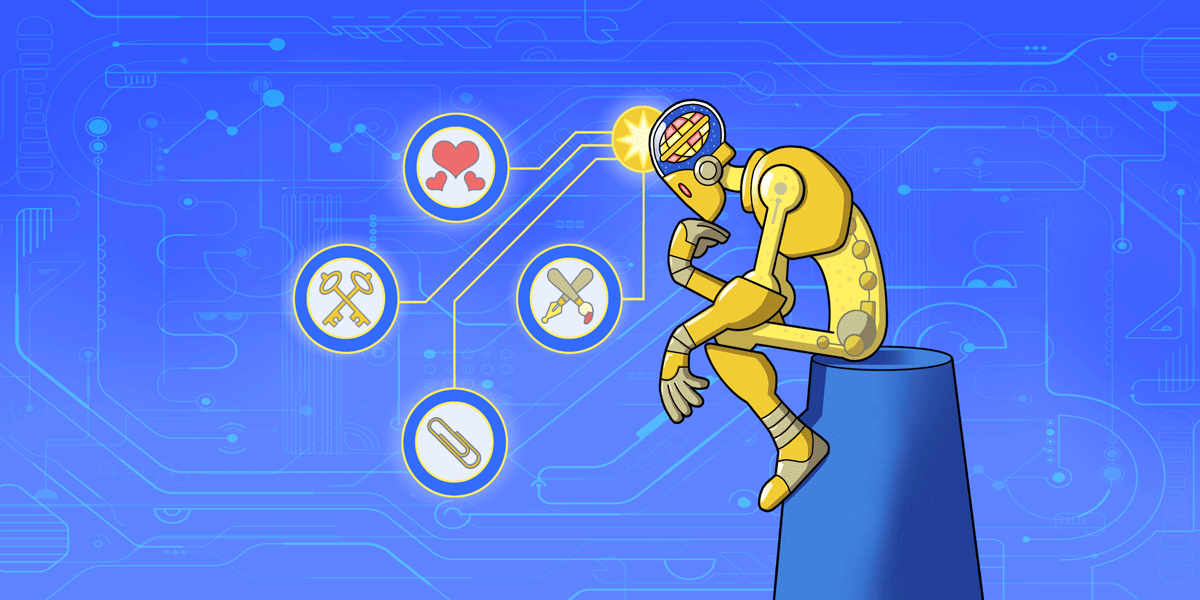
\includegraphics[width=11cm]{../pics/AI/eff-artificial-intelligence-ccby}
		\caption{The \citeauthor{eff17:ai} (EFF) questions whether patents will slow down innovations in AI (\citeyear{eff17:ai}) --credit: EFF}
	\end{figure}
}

\frame{
	\frametitle{Elon Musk does not want to block Innovation}
	\begin{figure}
		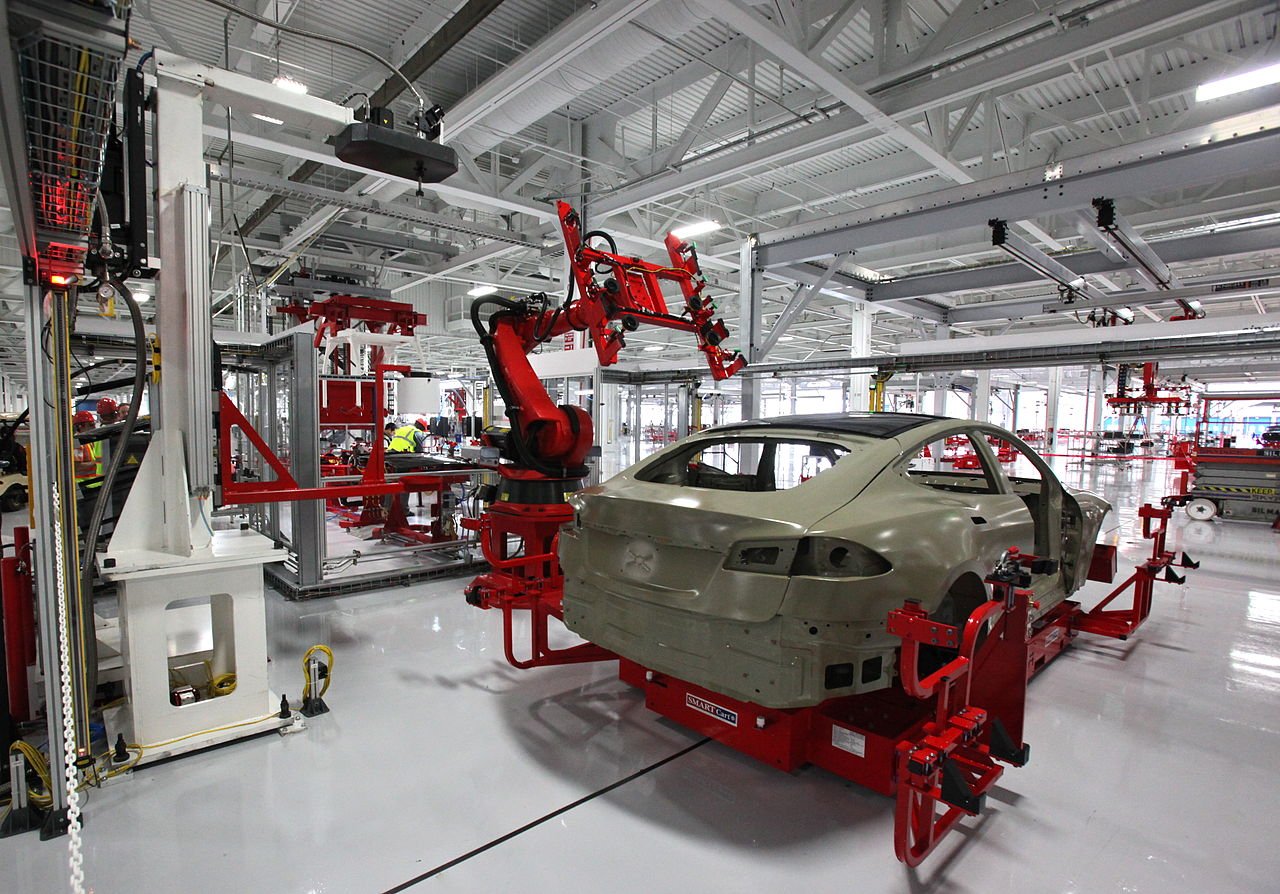
\includegraphics[height=6cm]{../pics/floss/1280px-Tesla_auto_bots}
		\caption{Tesla promises not to enforce patents (\cite{teslapatentstmt}) --credit: Steve Jurvetson}
		% https://commons.wikimedia.org/wiki/File:Tesla_auto_bots.jpg
	\end{figure}
}


% ======================================================================================================
%                         Blockchain and Open Source 
% ======================================================================================================
% 
\section{The case of Software}
\frame{
	\frametitle{A fight starting because of a Printer}
	\begin{figure}
		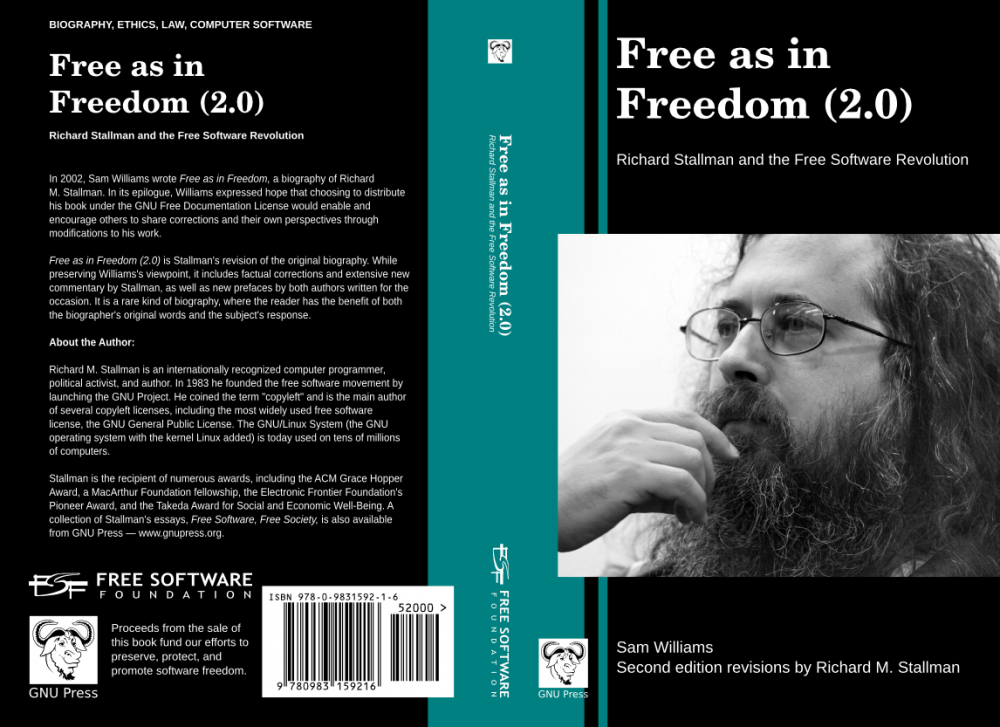
\includegraphics[height=6cm]{../pics/floss/productimage-picture-free-as-in-freedom-2-92}
		\caption{Richard Stallman's first step into Free Software (\cite{rms02:freedombook}; \cite{rms10:freedombook})}
	\end{figure}
}

\begin{frame}   % the four freedoms
	\frametitle{Free Software}
	\begin{figure}
		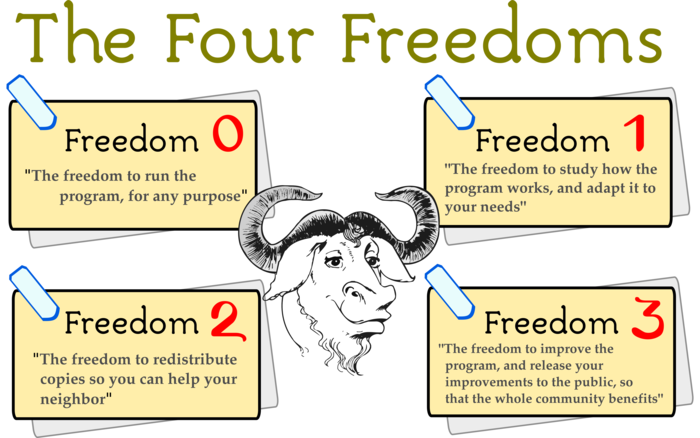
\includegraphics[width=11cm]{../pics/scaled_full_00c40105cea4c0aa3e9f}
	\end{figure}
\end{frame}

\begin{frame}
	\frametitle{Open Source runs (almost) Everything}
	\framesubtitle{2015 was an inflexion point}
	\begin{figure} % extracts from articles and other sources published on the Web
		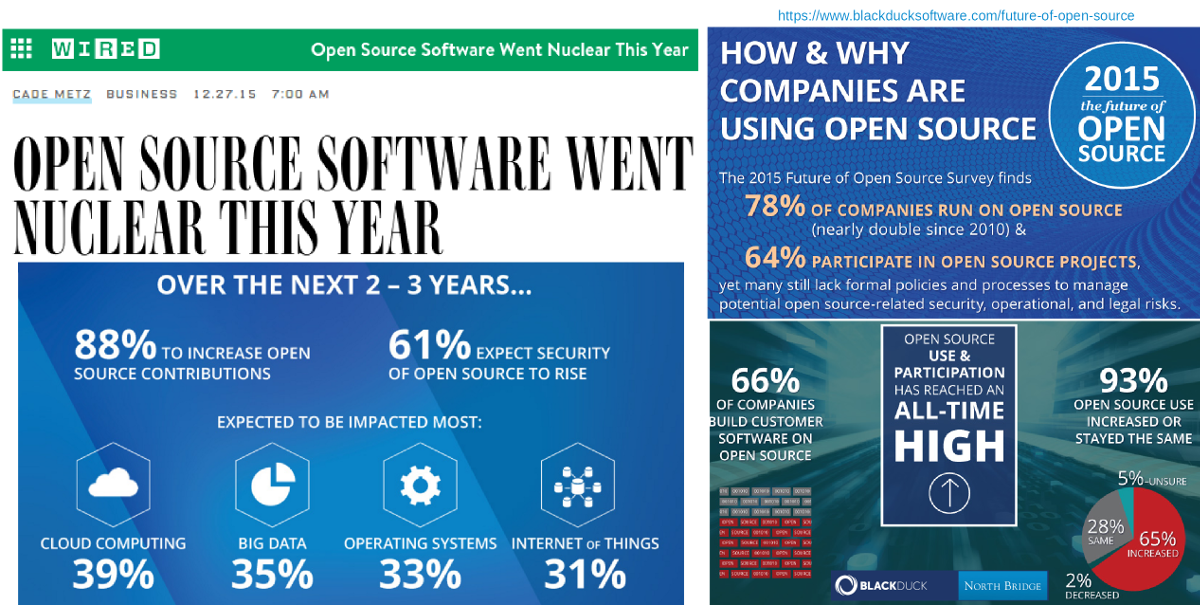
\includegraphics[width=11cm]{../pics/pic-open-source-went-nuclear-non-interlaced}
	\end{figure}
\end{frame}

\frame{
%	\frametitle{Free Software and Open Source Software}
	\frametitle{Building complex large-scale software systems (fast)}
%	\framesubtitle{An introduction to Free/Libre Open Source Software (\href{https://www.youtube.com/watch?v=Tyd0FO0tko8}{Intel, 2014})}
	\framesubtitle{An introduction to Free/Libre Open Source Software (\cite{intel2014:FLOSS})}
	\begin{figure}
	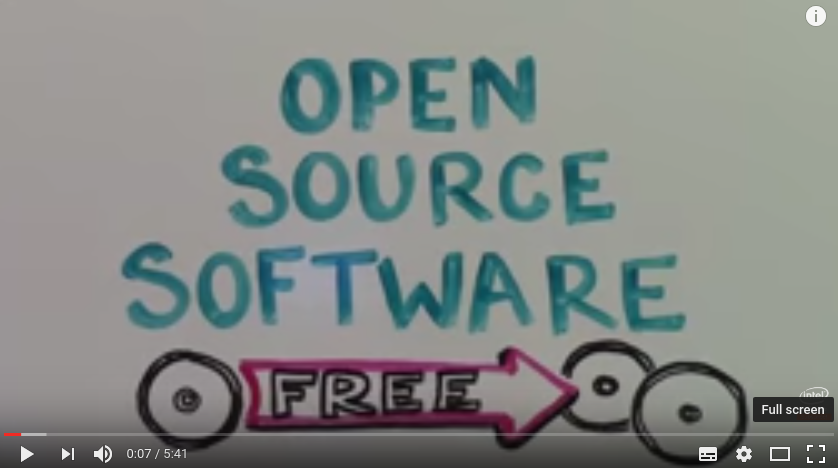
\includegraphics[height=5cm]{../pics/intel-FLOSS-intro}
	\caption{\url{https://www.youtube.com/watch?v=Tyd0FO0tko8}}
	\end{figure}
	\tiny \copyright \href{https://www.youtube.com/watch?v=Tyd0FO0tko8}{Intel Software (2014)}
}

\frame{
	\frametitle{Nadia Eghbal's report (\citeyear{eghbal2016})}
	\framesubtitle{Roads and Bridges: The Unseen Labor Behind Our Digital Infrastructure}
	\begin{columns}
	\column{0.3\textwidth}
		\begin{figure}
		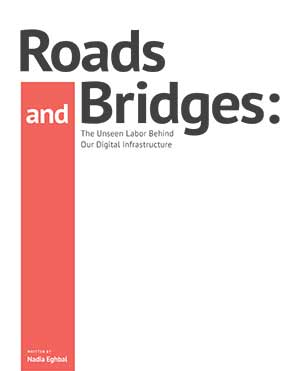
\includegraphics[width=3cm]{../pics/logos/roads-and-bridges}
		\end{figure}
	\column{0.7\textwidth}
	\begin{itemize}
        \item Open Source Software runs core infrastructure services
        \item It is poorly funded (e.g. OpenSSL)
        \item Who should fund roads and bridges?
    \end{itemize}
	\end{columns}
}

\frame{
	\frametitle{Blockchain is Open/Free by design}
	\begin{figure}
	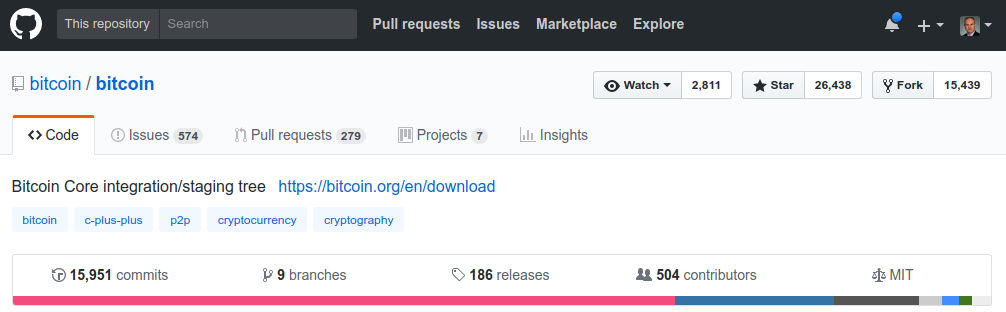
\includegraphics[width=10cm]{../../pics/bitcoin-core-github}
	%
\includegraphics[width=8cm,left]{../../pics/bitcoin-core-github-license}
	
\includegraphics[width=10cm]{../../pics/bitcoin-core-github-license}
	\end{figure}
}

\frame{
	\frametitle{Starting your own Free/Libre Open Source Software project}
    \framesubtitle{Nicely summarized by Roberto Di~Cosmo (\citeyear{dicosmo:achieving-impact})}
	\begin{figure}
	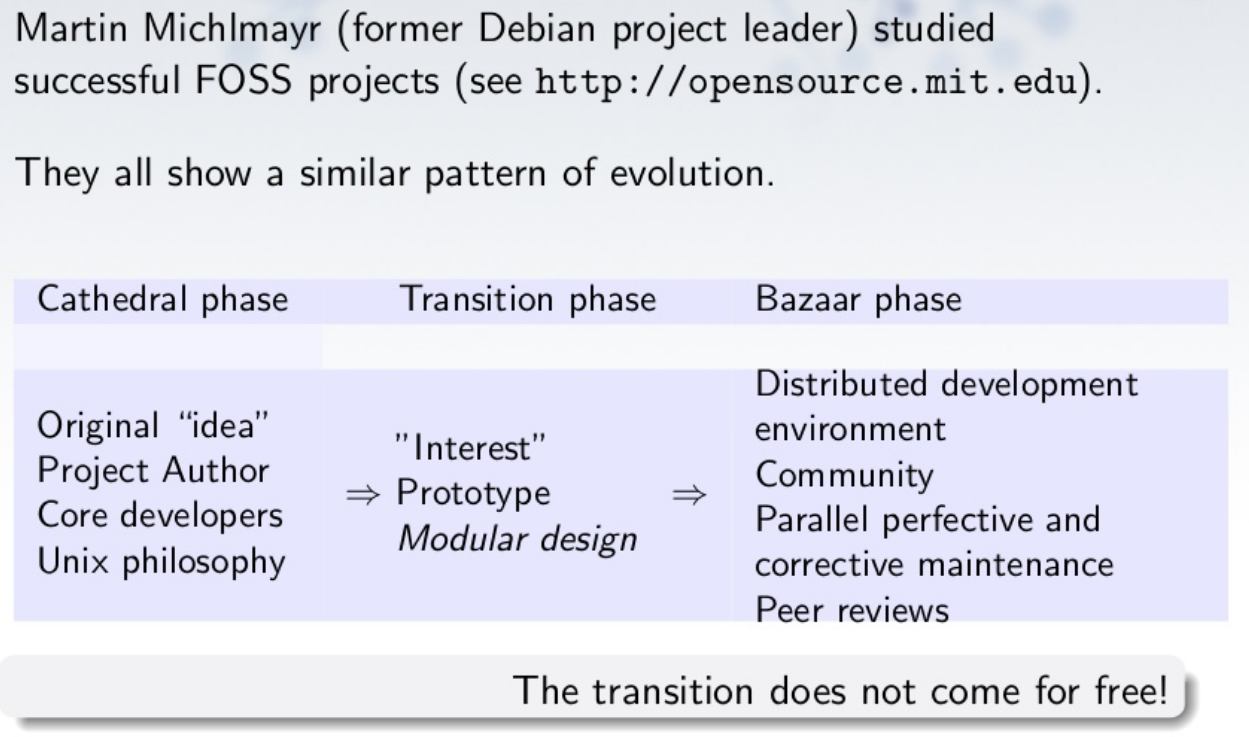
\includegraphics[width=7cm]{../../pics/dicosmo-successful-project}
	\end{figure}
	\begin{itemize}
        \pause
        \item Identify a need
        \pause
        \item Build a prototype
        \pause
        \item Grow a community
        \pause
        \item Set up an ecosystem \\
                (users, developers, architects, designers, service providers...)
% the last two are the most difficult
    \end{itemize}
}


% ======================================================================================================
%                         Blockchain and Open Source 
% ======================================================================================================
% 
\section{Tokenization and the Blockchain}

%----------------------------------------------------------------------------

\subsection{Market size}

\frame{
    \frametitle{Top industries and blockchain use-cases}
    \framesubtitle{According to \citeauthor{idc2018:spendingforecast} (\citeyear{idc2018:spendingforecast})}
    \begin{itemize}
        \item financial sector (\$552 million in 2018) --custody and asset tracking, trade finance, in addition to cross-border payments and settlements
        \item distribution and services sector (\$379 million in 2018) --asset/goods management and lot lineage/provenance
        \item manufacturing and resources sector (\$334 million in 2018) --as above
    \end{itemize}
}

\frame{
    \frametitle{Market size for blockchain applications}
	\begin{figure}
		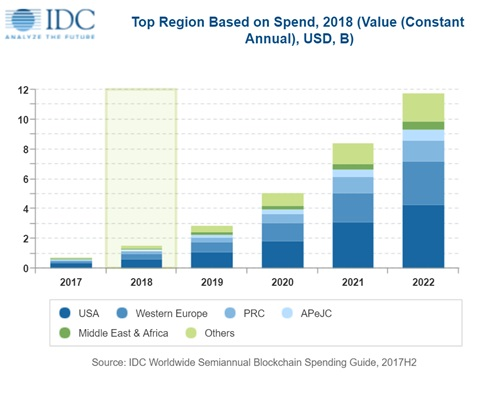
\includegraphics[height=6cm]{../pics/blockchain/idc2018-spendingforecast}
    \caption{from \citeauthor{idc2018:spendingforecast} (\citeyear{idc2018:spendingforecast})}
	\end{figure}
}

%----------------------------------------------------------------------------
\subsection{Features}

\frame{
	\frametitle{Top advantages per industry}
	\begin{figure}
		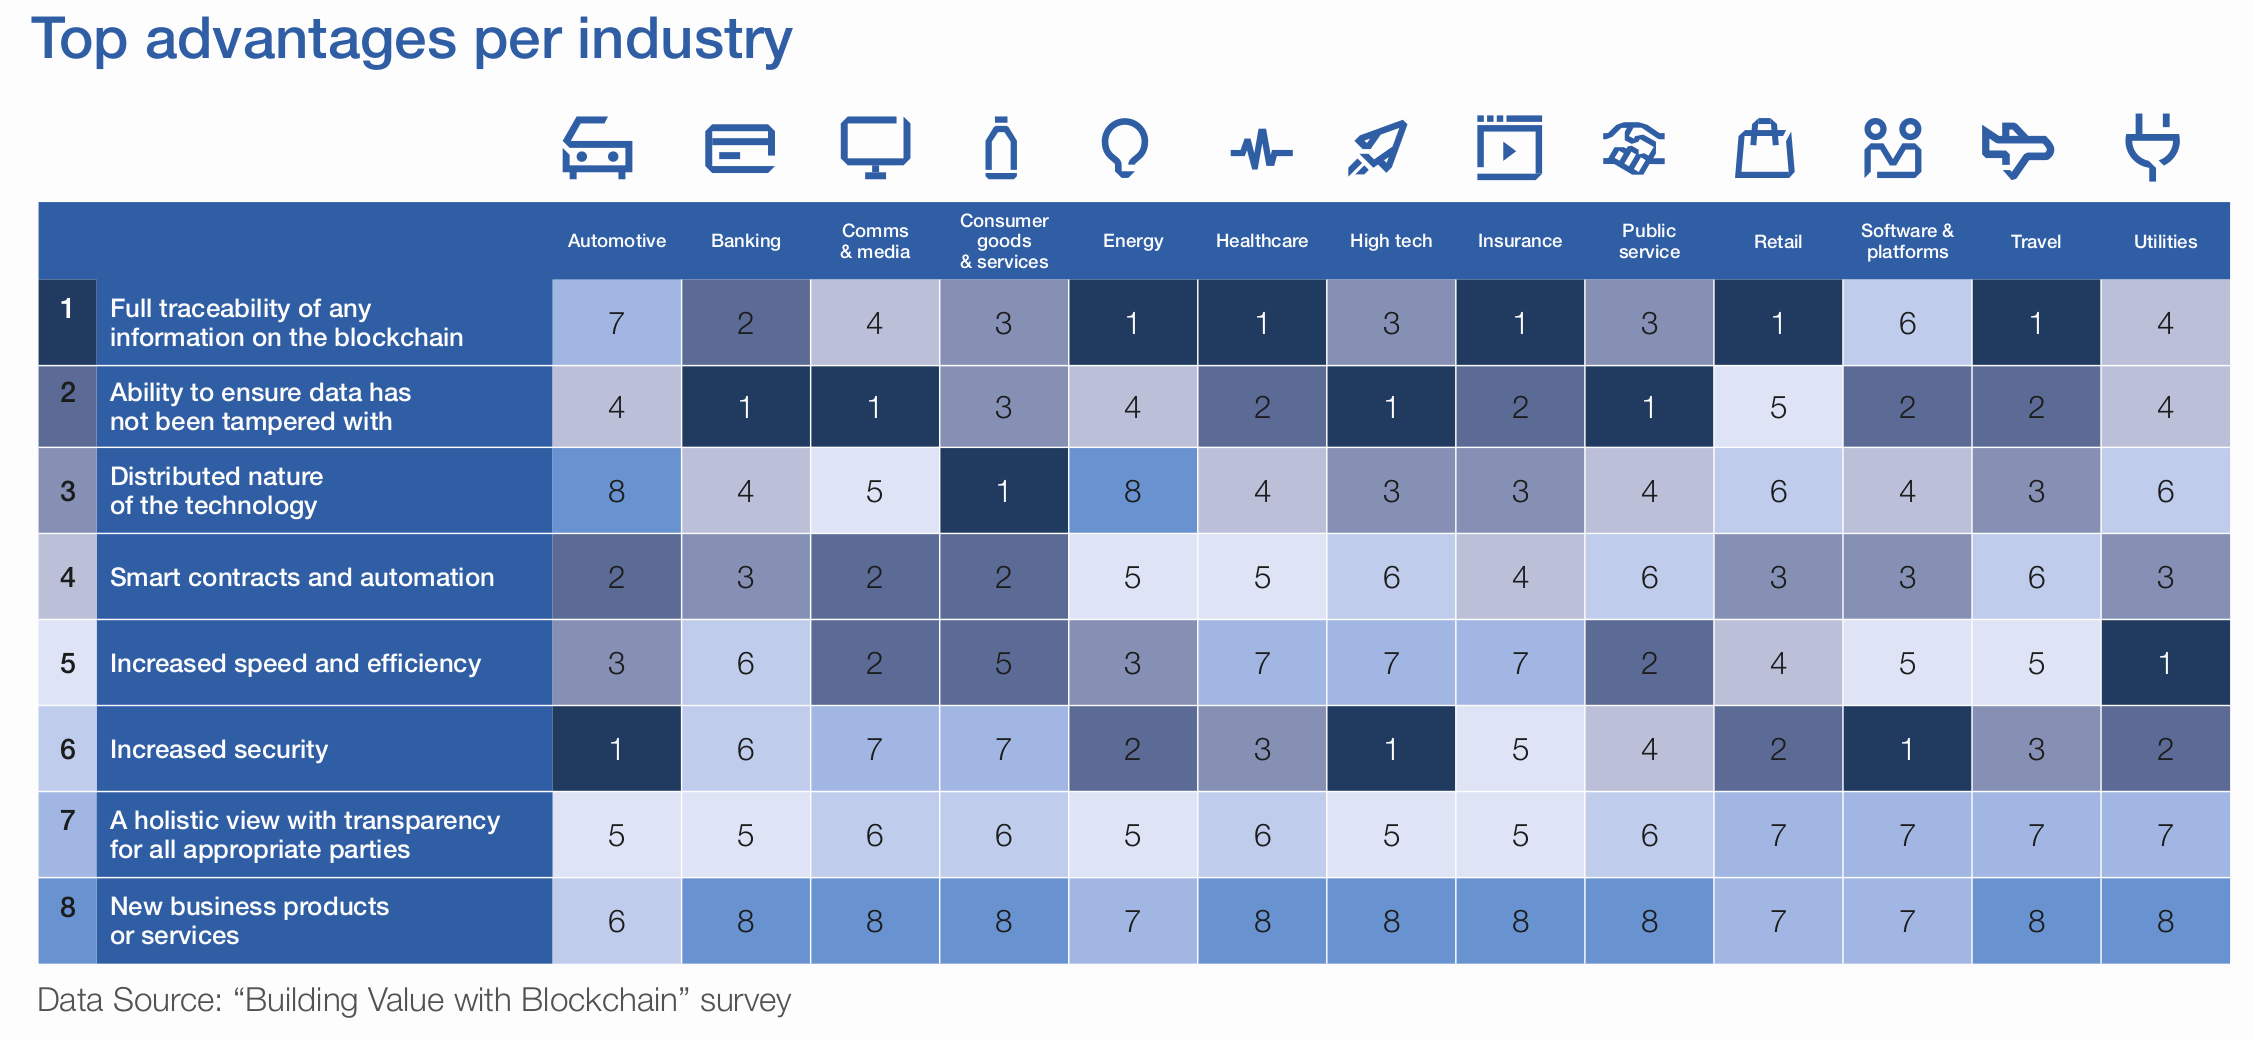
\includegraphics[width=11.5cm]{../pics/blockchain/wef-accenture201906-topadvantage}
    \caption{from the \citeauthor{wef-accenture201906} (\citeyear{wef-accenture201906})}
	\end{figure}
% based on a global survey of 550 individuals across 13 industries, dozens of interviews with public-sector leaders and private-sector chief executive officers, and an analysis of 79 blockchain projects. The projects were evaluated across three main value dimensions: 1) improving productivity and quality; 2) increasing transparency among parties; and 3) reinventing  products and processes.
% (...)
% When asked what led organizations to invest in blockchain technology, 75% included their organizational priority for innovation. The top three areas of interest across surveyed industries were: 1) full traceability of information on the blockchain; 2) the ability to check that data had not been tampered with; and 3) the way the technology is distributed. Notably, few organizations selected “new business products or services” – which ranked last among the options for investment.
}

\frame{
	\frametitle{WEF's Blockchain Value Framework}
	\begin{figure}
		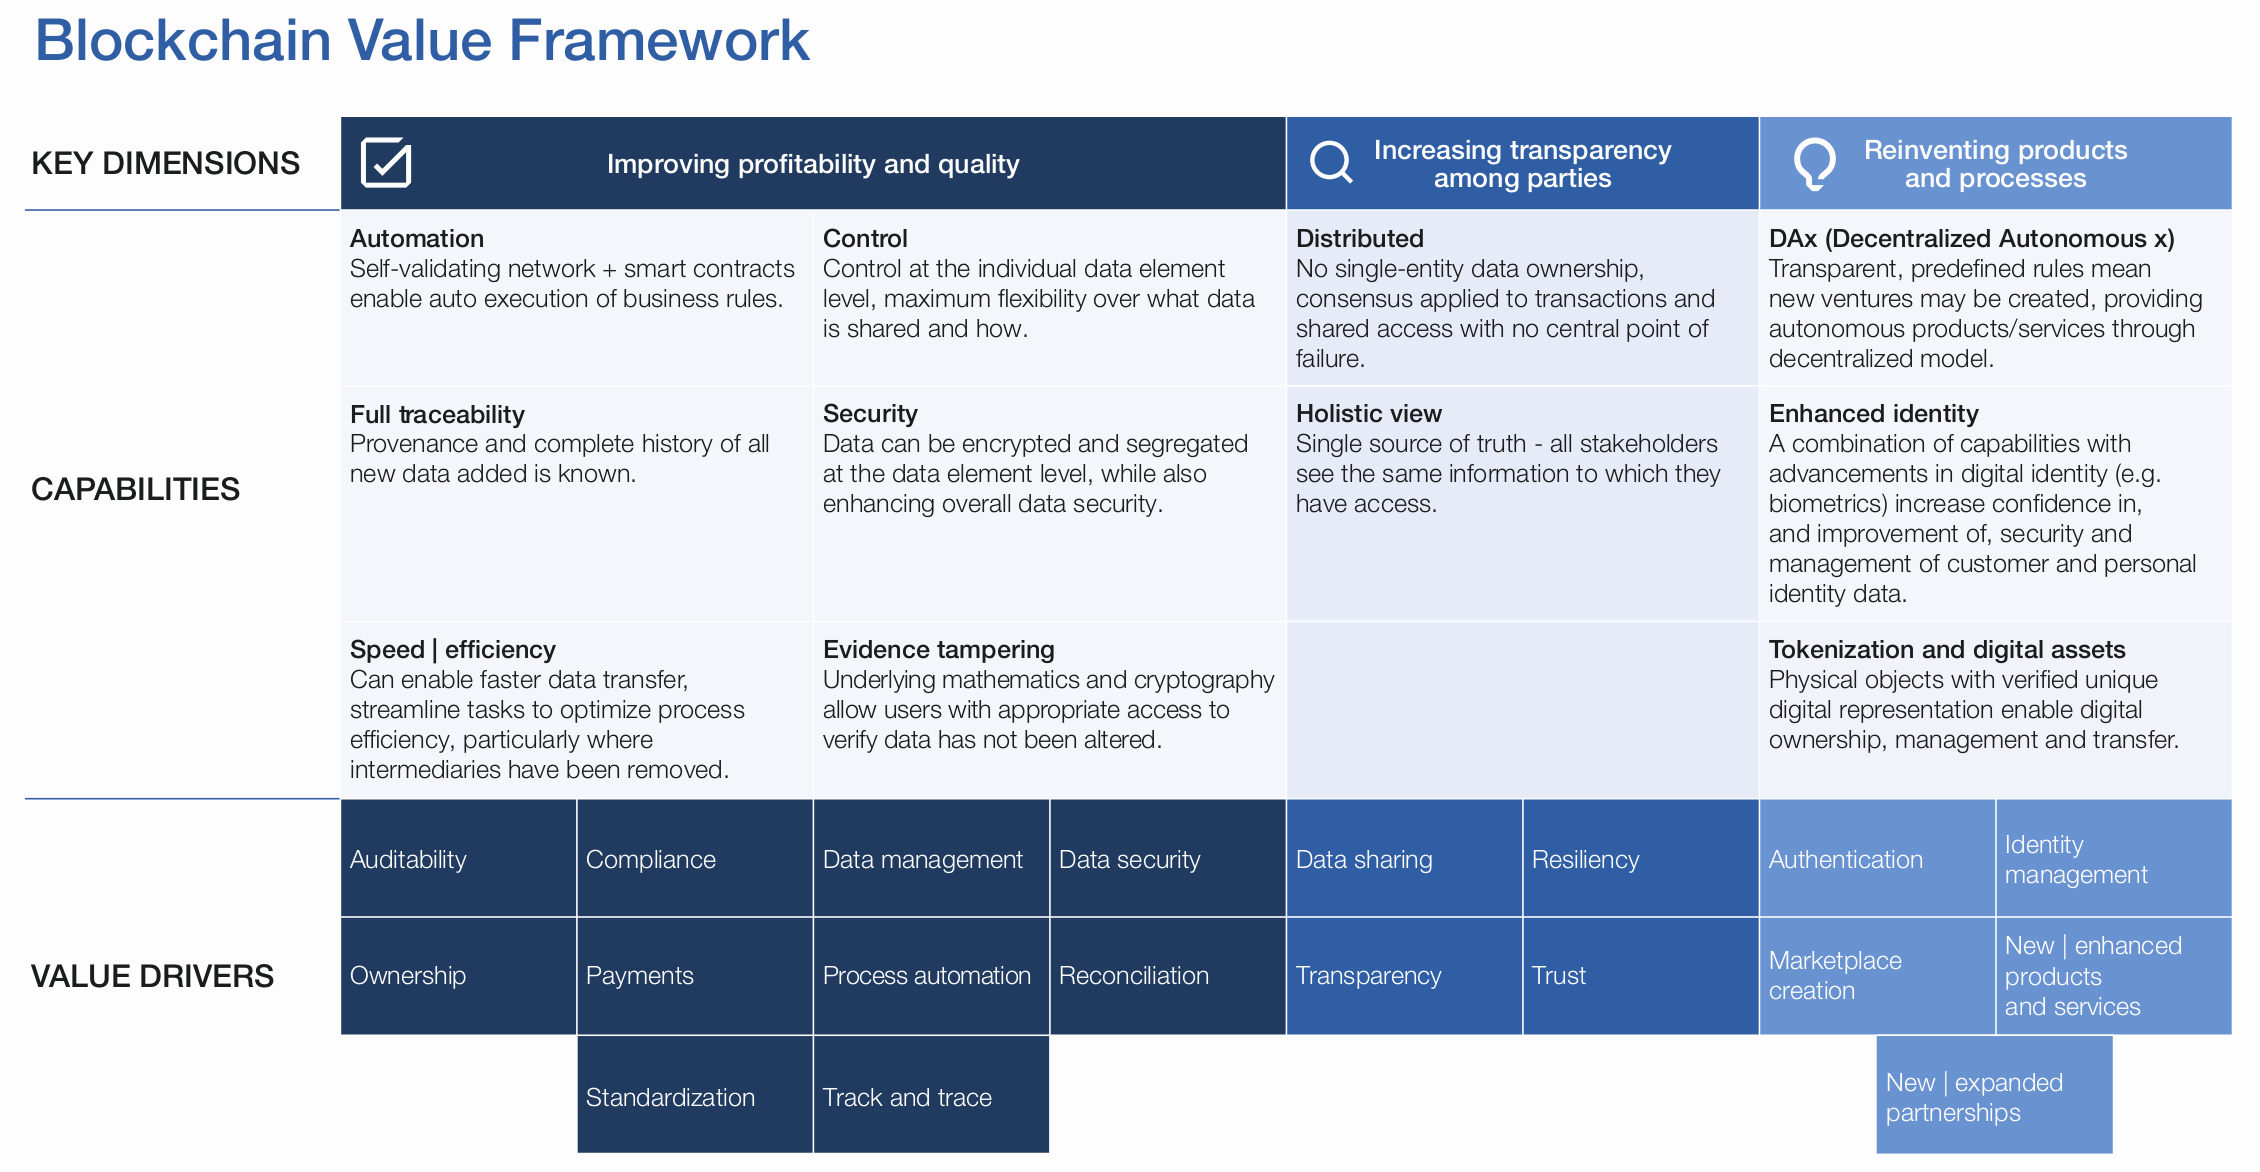
\includegraphics[width=11.5cm]{../pics/blockchain/wef-accenture201906-value-fwk}
    \caption{from the \citeauthor{wef-accenture201906} (\citeyear{wef-accenture201906})}
	\end{figure}
}

%----------------------------------------------------------------------------
\subsection{Use-cases in Identity Management}
\frame{
	\frametitle{Pan-Canadian Trust Framework | Cadre de Confiance pancanadien}
	\framesubtitle{\url{https://canada-ca.github.io/PCTF-CCP/}}
	\begin{figure}
		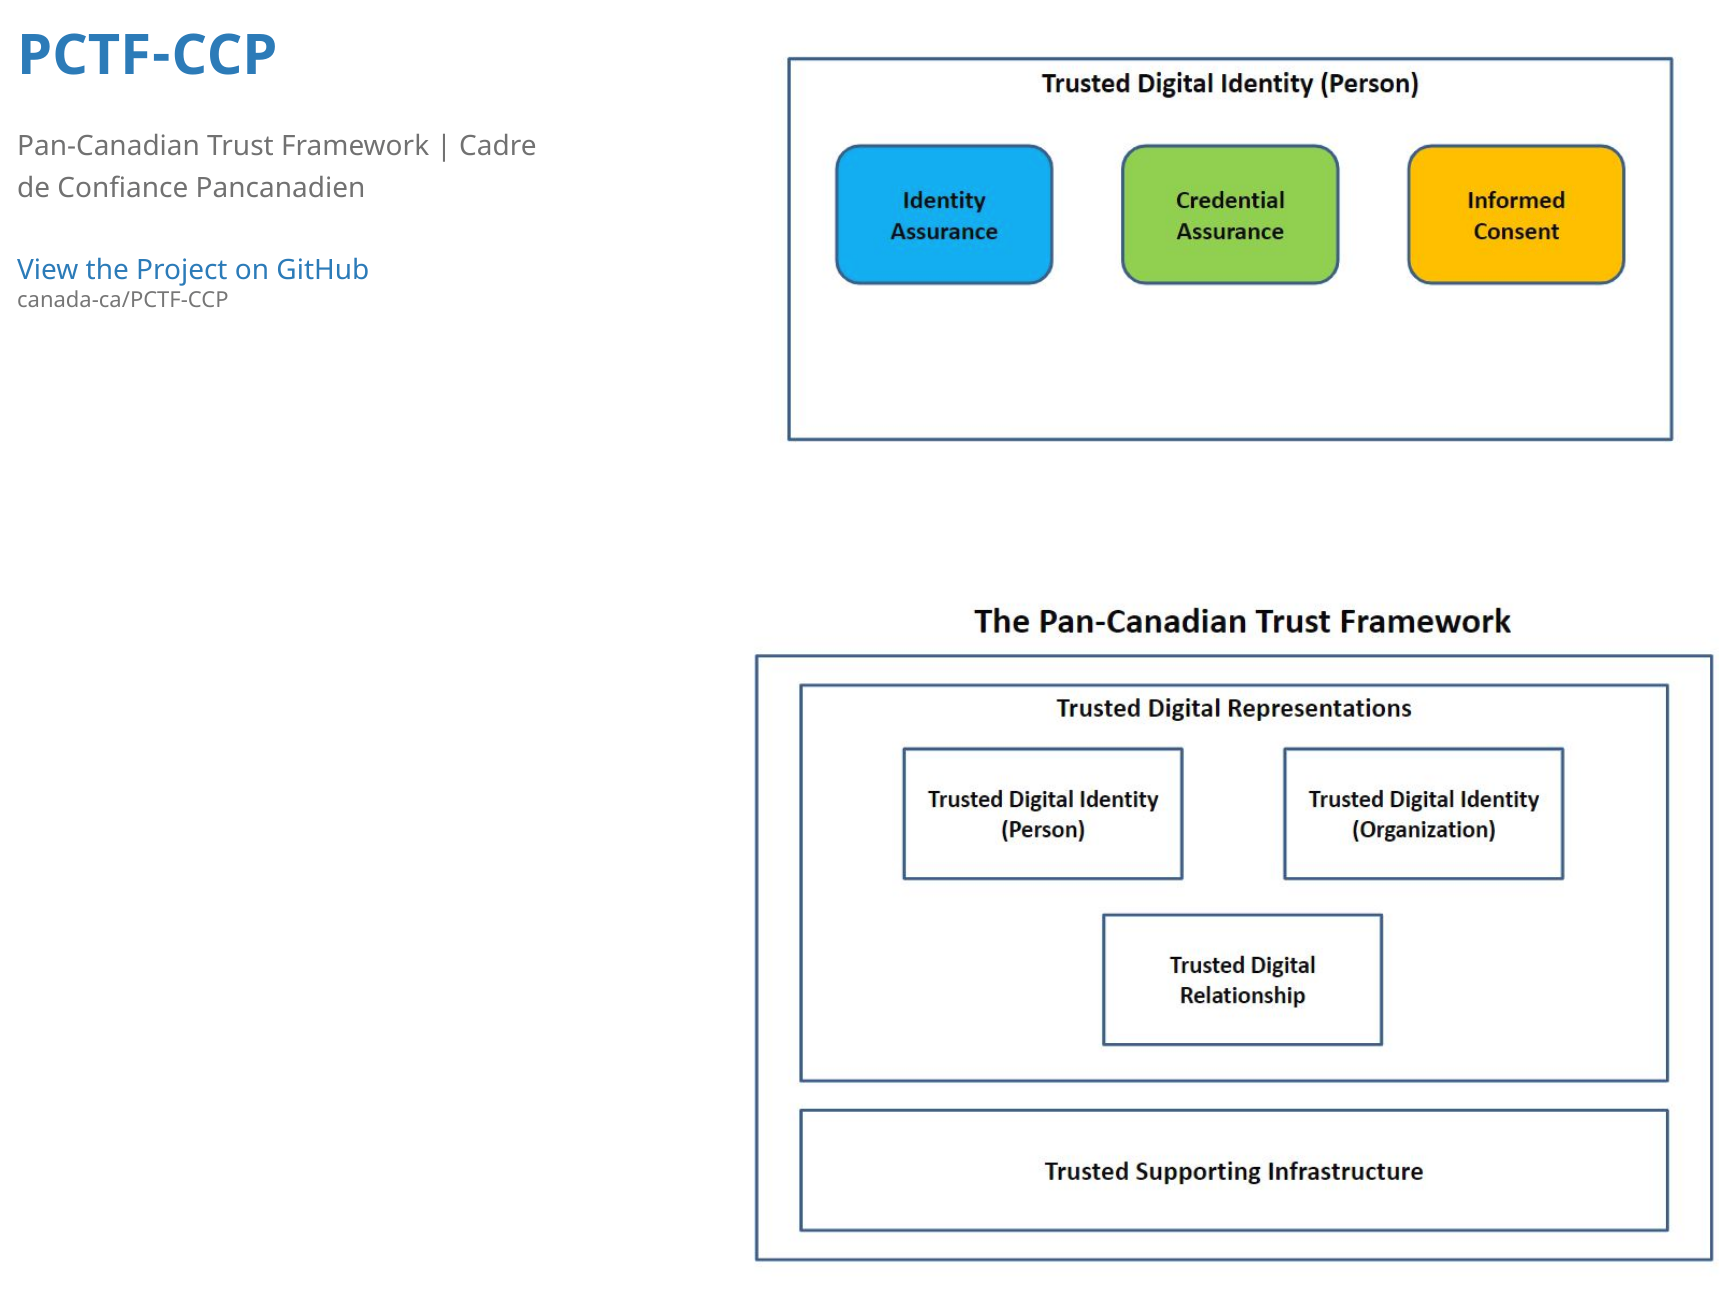
\includegraphics[height=6cm]{../pics/identity/pctf}
	\end{figure}
}

\frame{
	\frametitle{}
	\centering\Huge
	uPort 
}

\frame{
	\frametitle{uPort stack vs ERC-725}
	\begin{figure}
		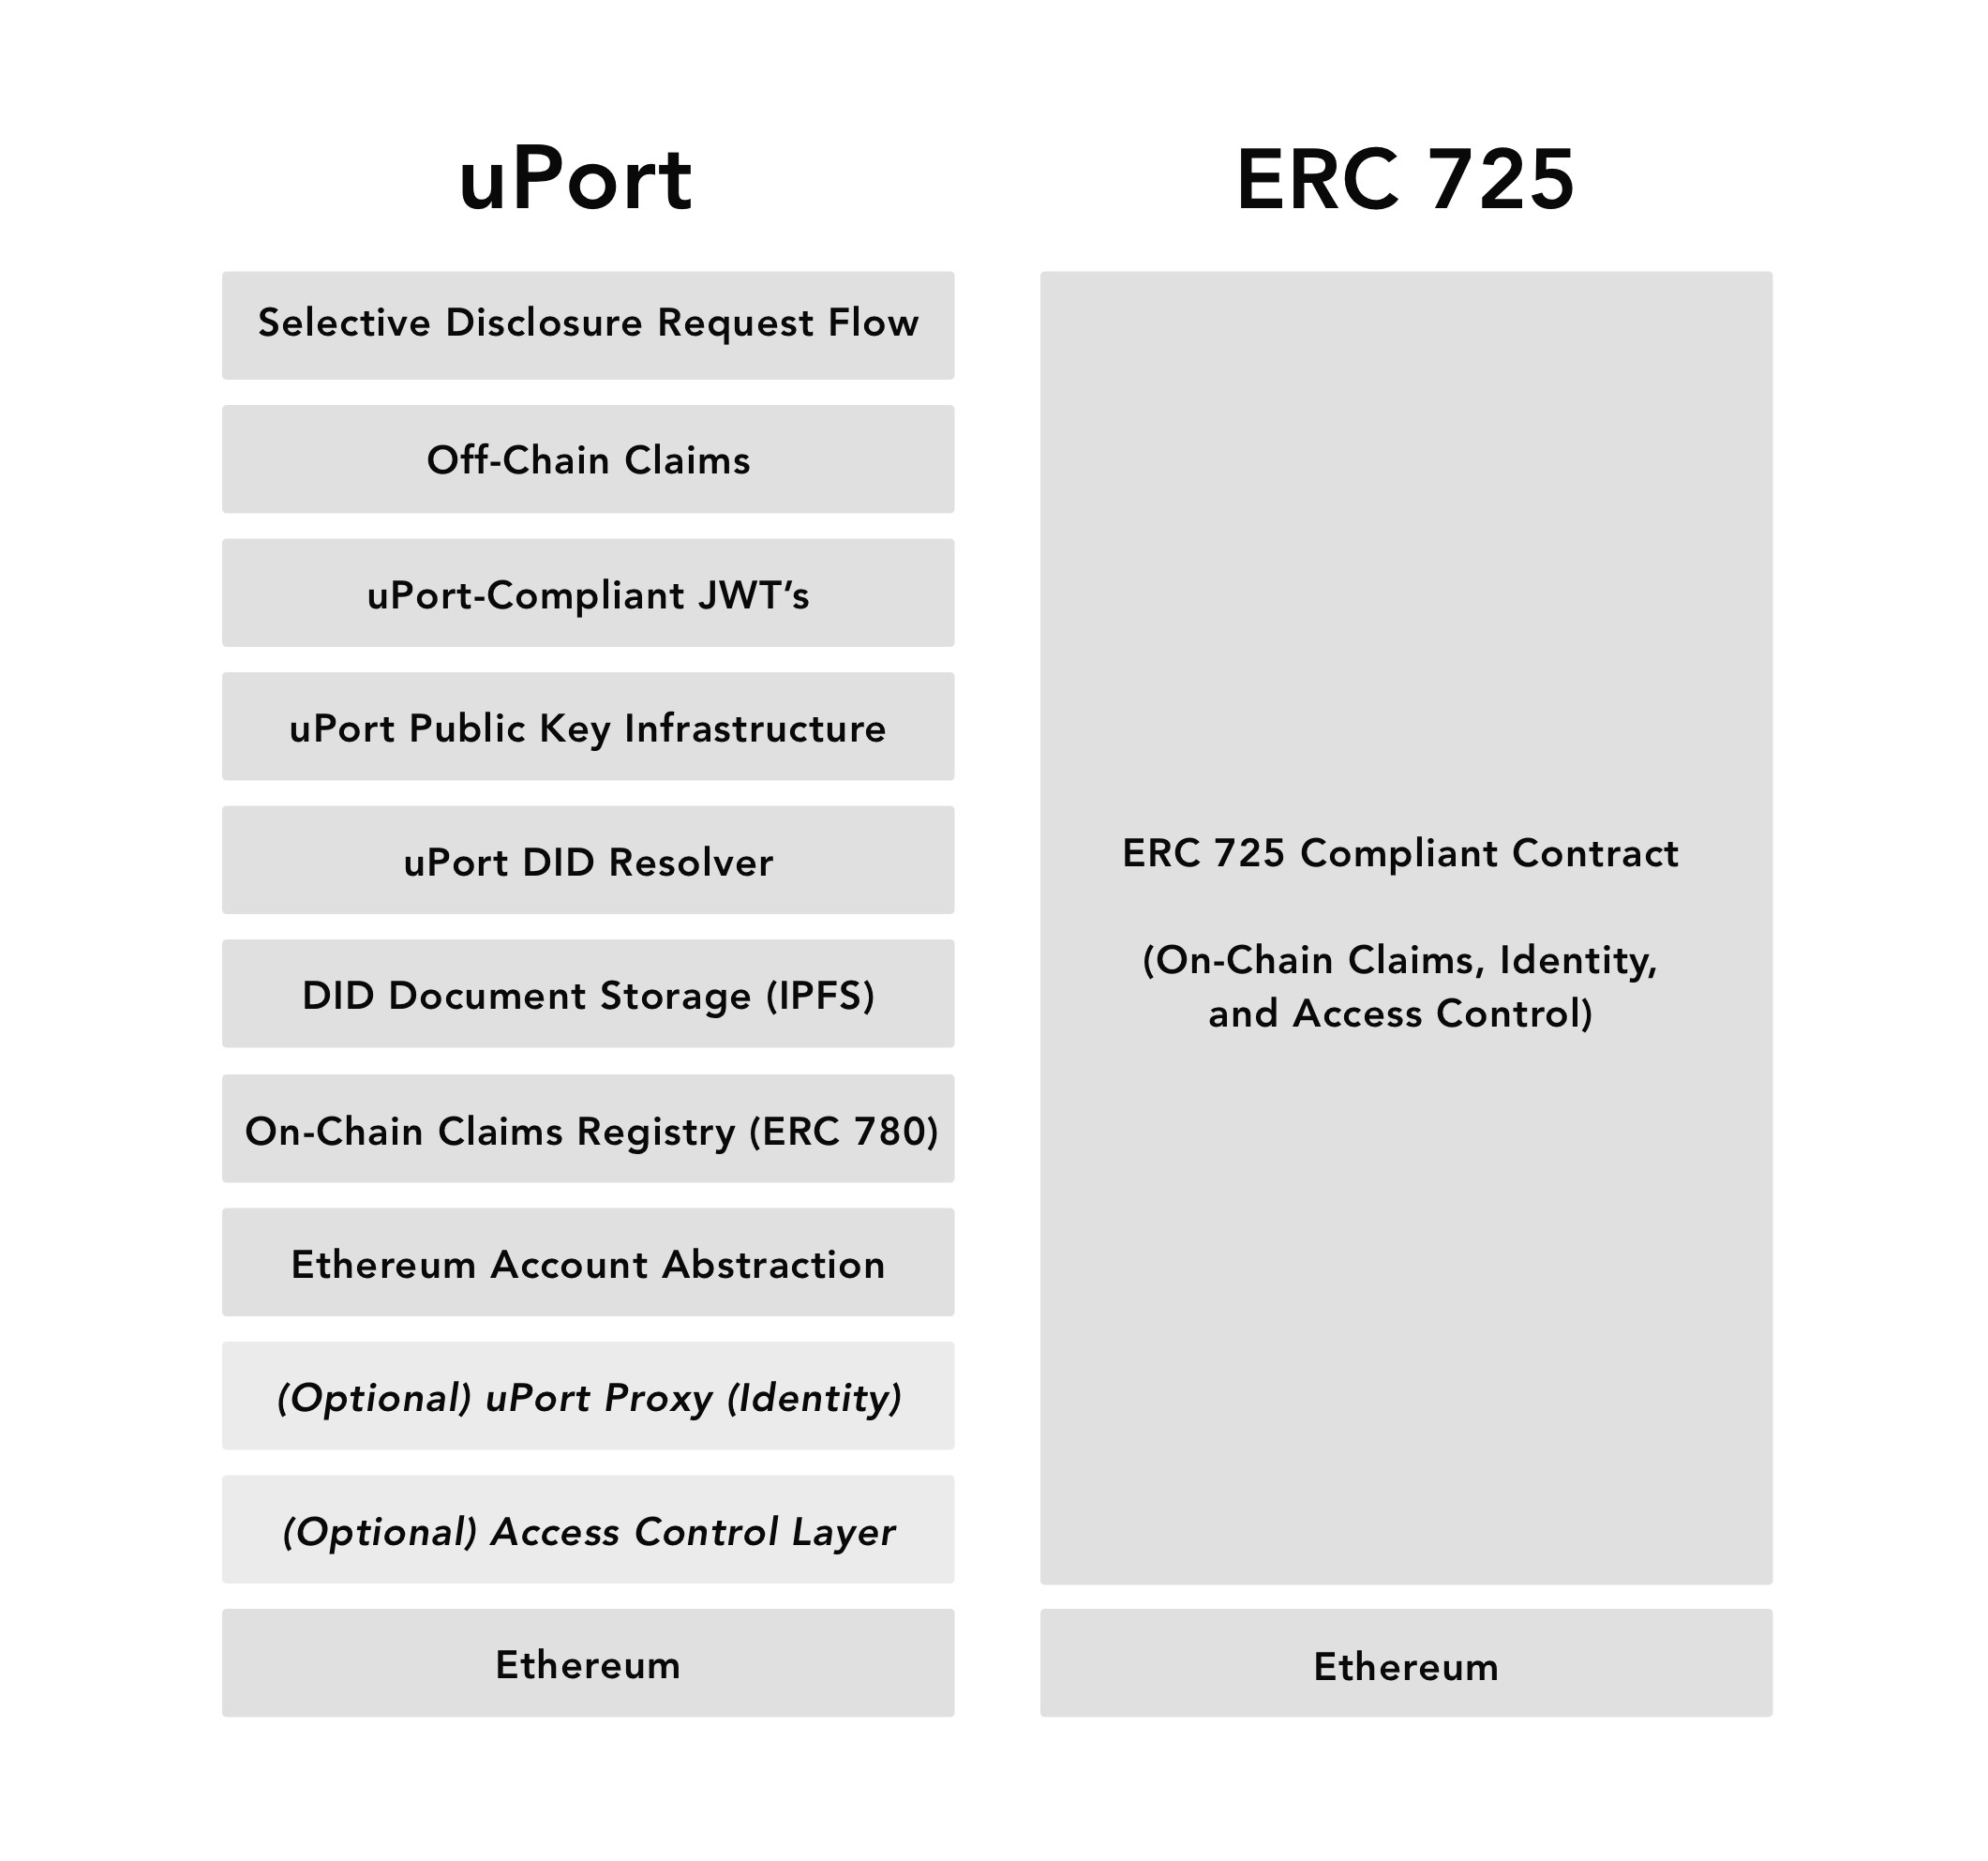
\includegraphics[height=6cm]{../pics/identity/uport-erc-725}
			\captionsetup{justification=centering}
			\caption{from \cite{uport201801:standards}}
	\end{figure}
}

\frame{
	\frametitle{The first e-bike service worldwide powered by decentralized identity}
	\framesubtitle{See full article from \cite{nawfal2019:uport-bike}}
	% https://medium.com/uport/zug-residents-can-now-ride-e-bikes-using-their-uport-powered-zug-digital-ids-7ed31ac9d621
	% see also Zug eID launch -- https://www.ethnews.com/zug-and-uport-see-first-citizens-identity-registered-on-the-ethereum-blockchain
	\begin{figure}
		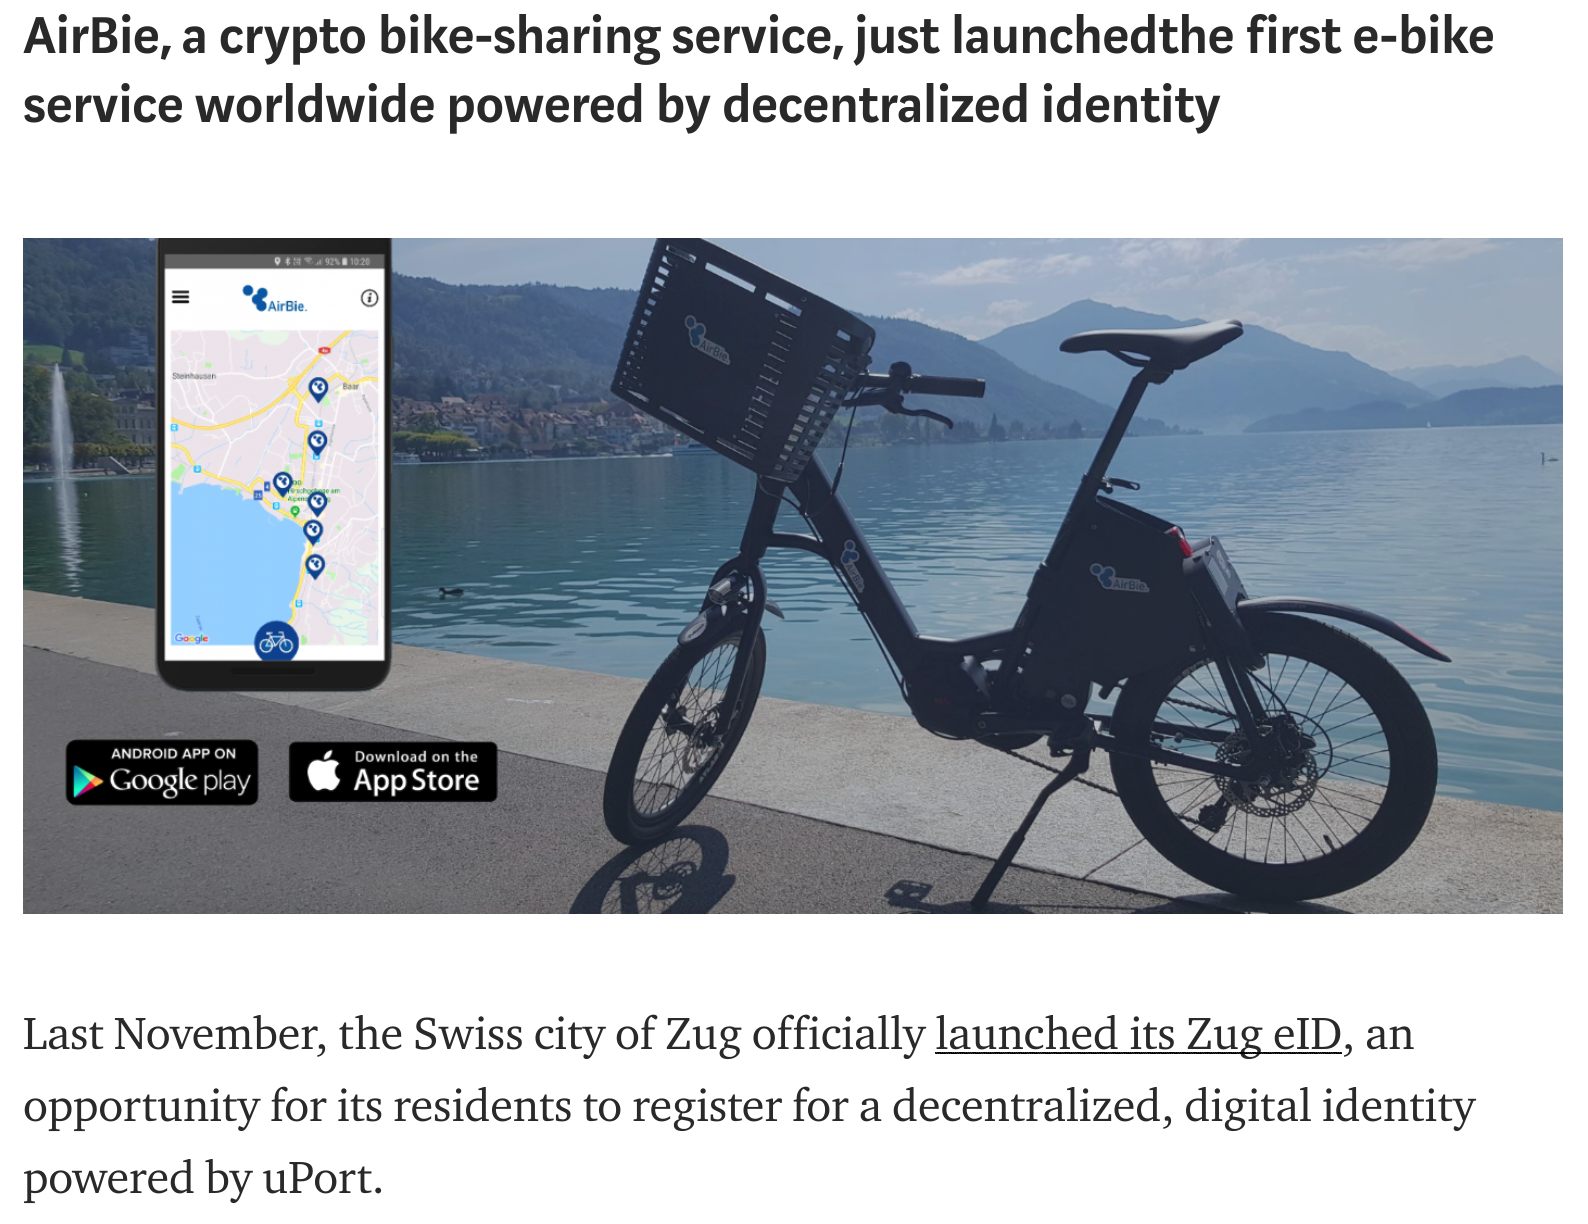
\includegraphics[height=6cm]{../pics/identity/uport-bike}
	\end{figure}
}

\frame{
	\frametitle{}
	\centering\Huge
	Sovrin -- Hyperledger Indy
}

\frame{
	\frametitle{Self-Sovereign Identity}
	\framesubtitle{Extract from the white paper from \cite{sovrin-white-paper}}
	\begin{figure}
		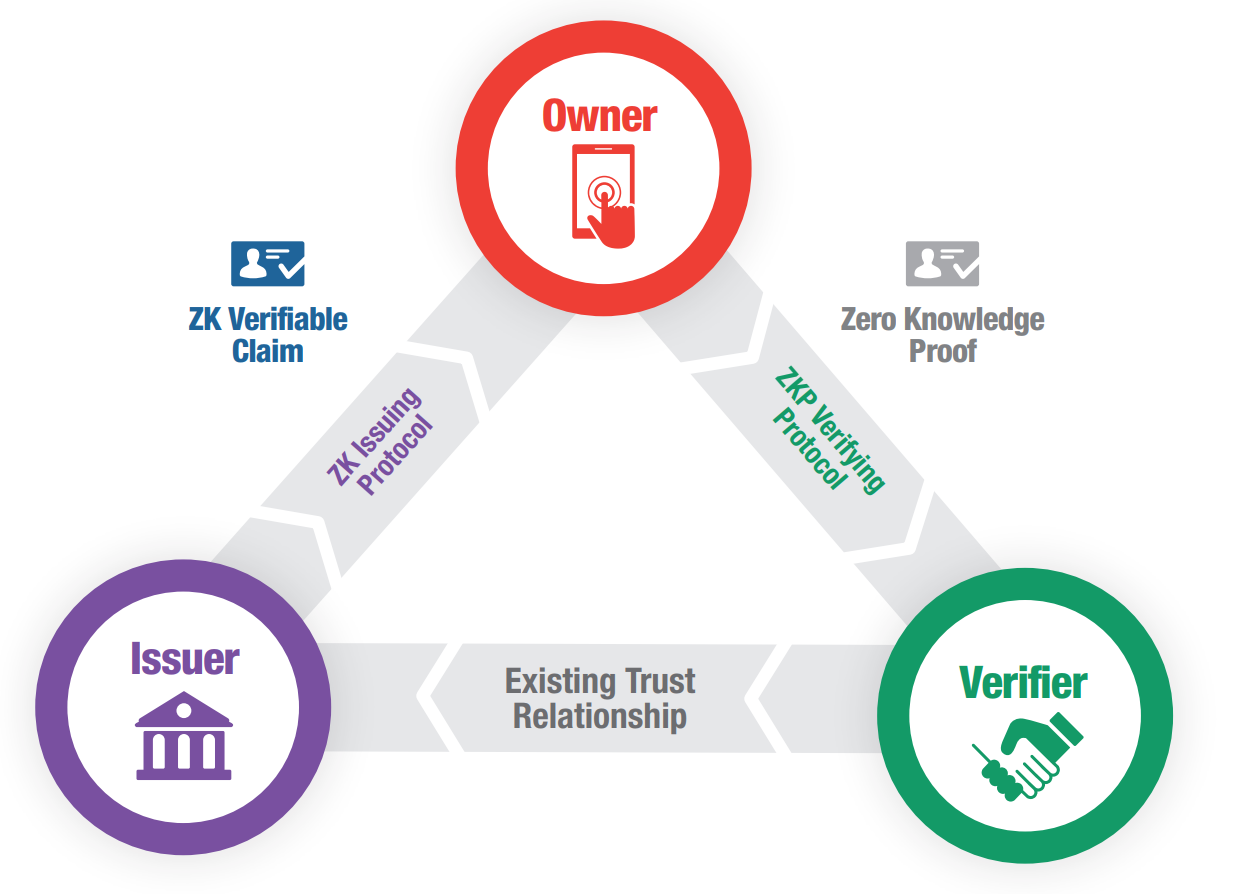
\includegraphics[height=6cm]{../pics/identity/sovrin-zkp}
	\end{figure}
}

\frame{
	\frametitle{The Verifiable Organizations Network (VON)}
	\framesubtitle{\url{https://vonx.io}}
	\begin{figure}
		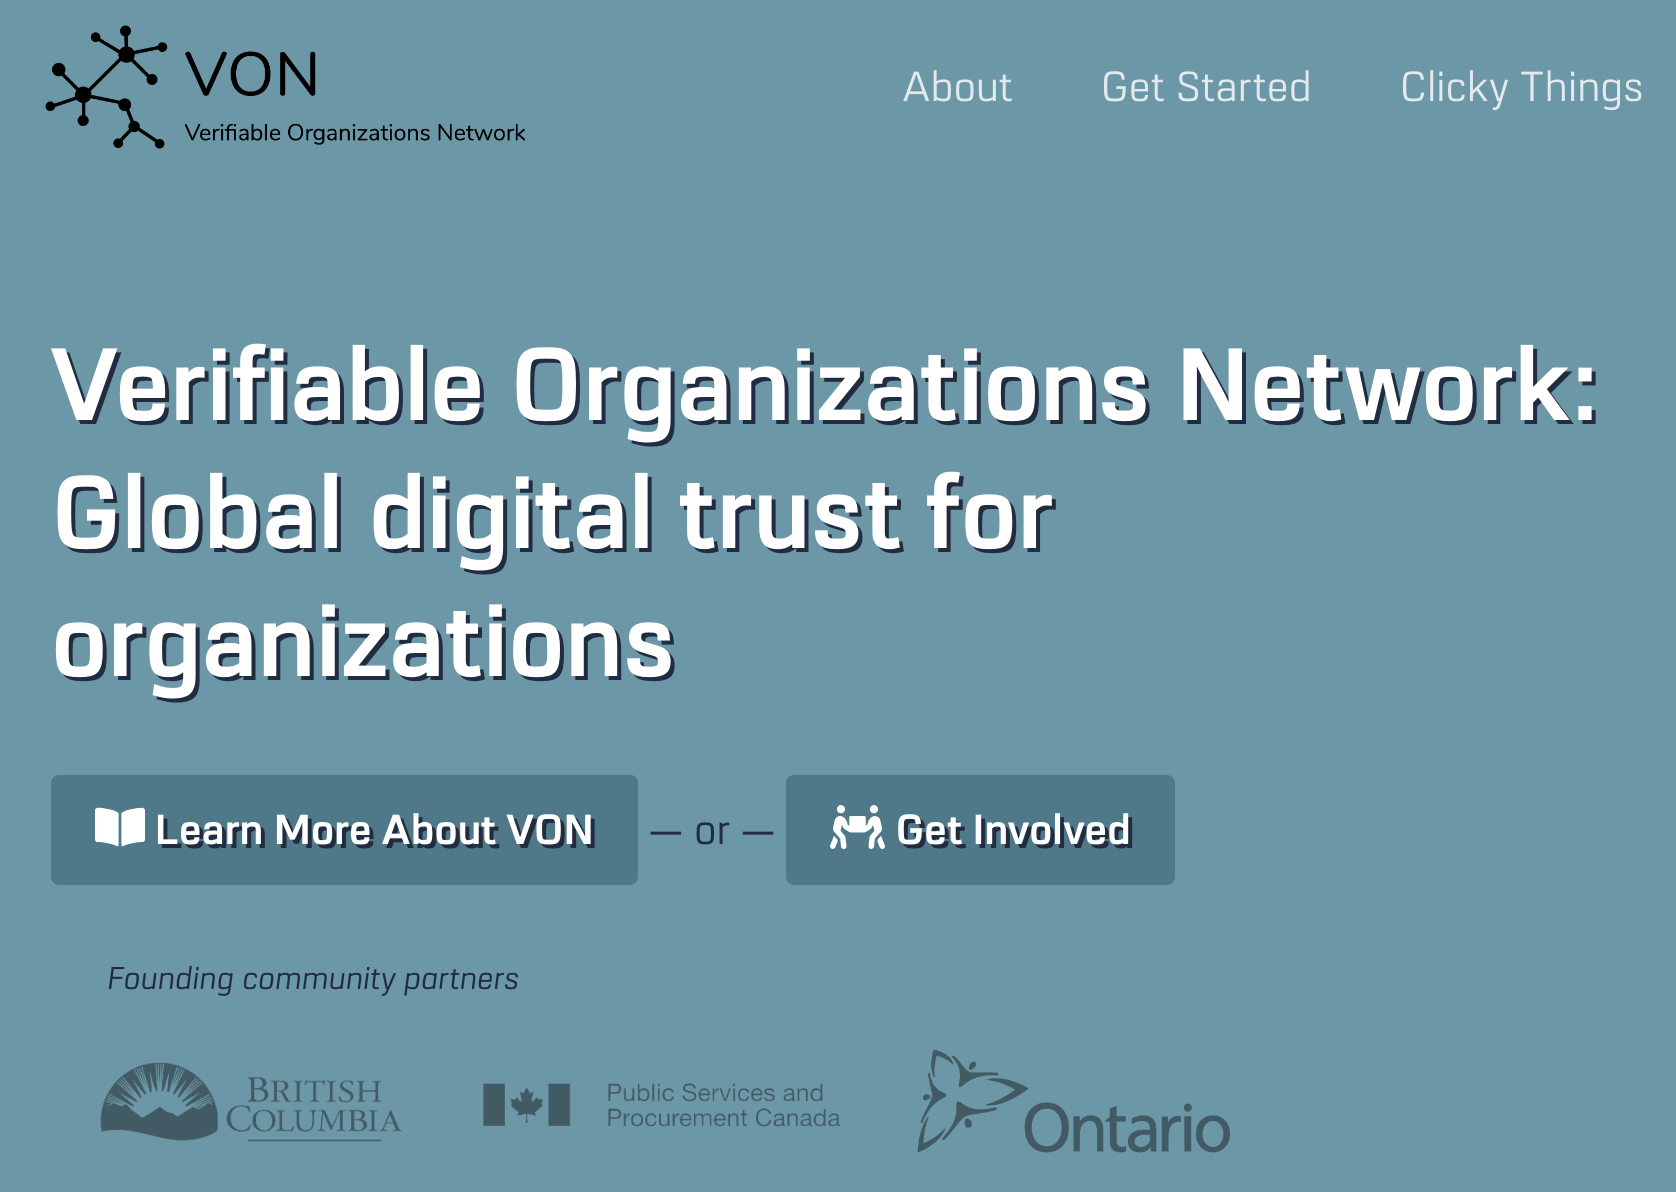
\includegraphics[height=6cm]{../pics/identity/vonx}
	\end{figure}
}

\frame{
	\frametitle{SSI in Alberta}
	\begin{figure}
		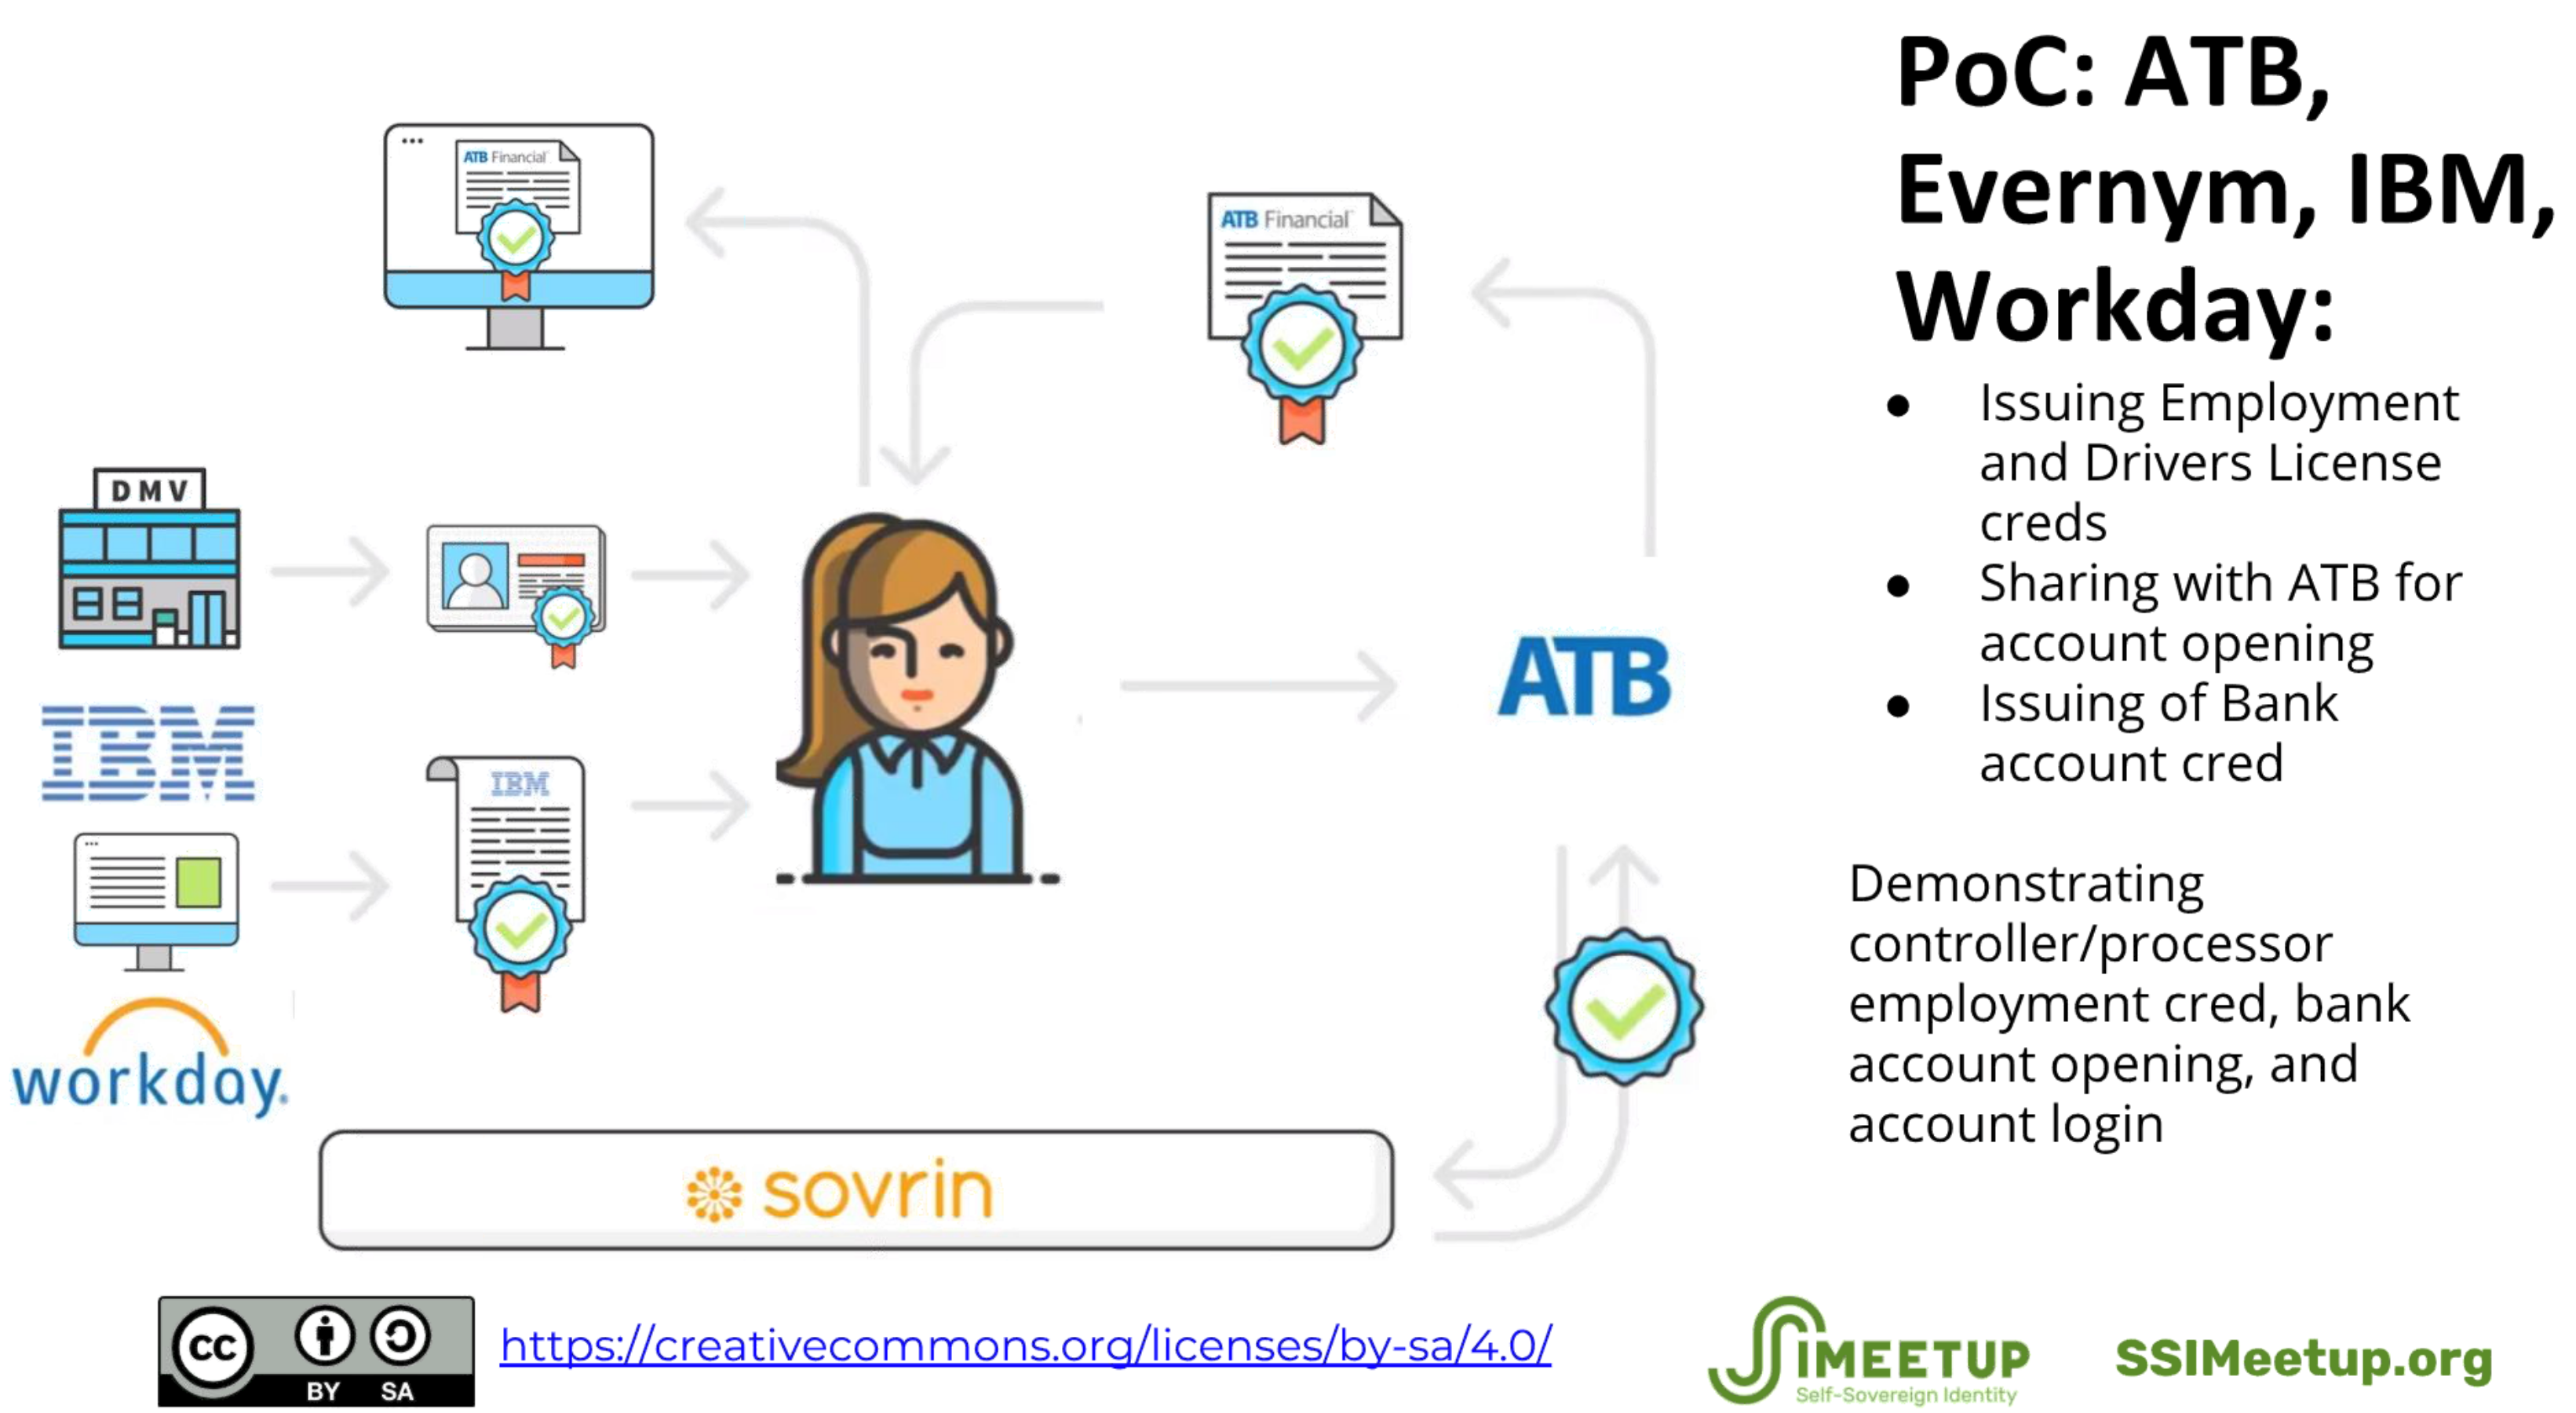
\includegraphics[height=6cm]{../pics/case_studies/atb-evernym-ibm-workday}
		\captionsetup{justification=centering}
		\caption{from \cite{ssimeetup201902:atb-slides}}
	\end{figure}
}

\frame{
	\frametitle{SSI in Alberta}
	\begin{figure}
		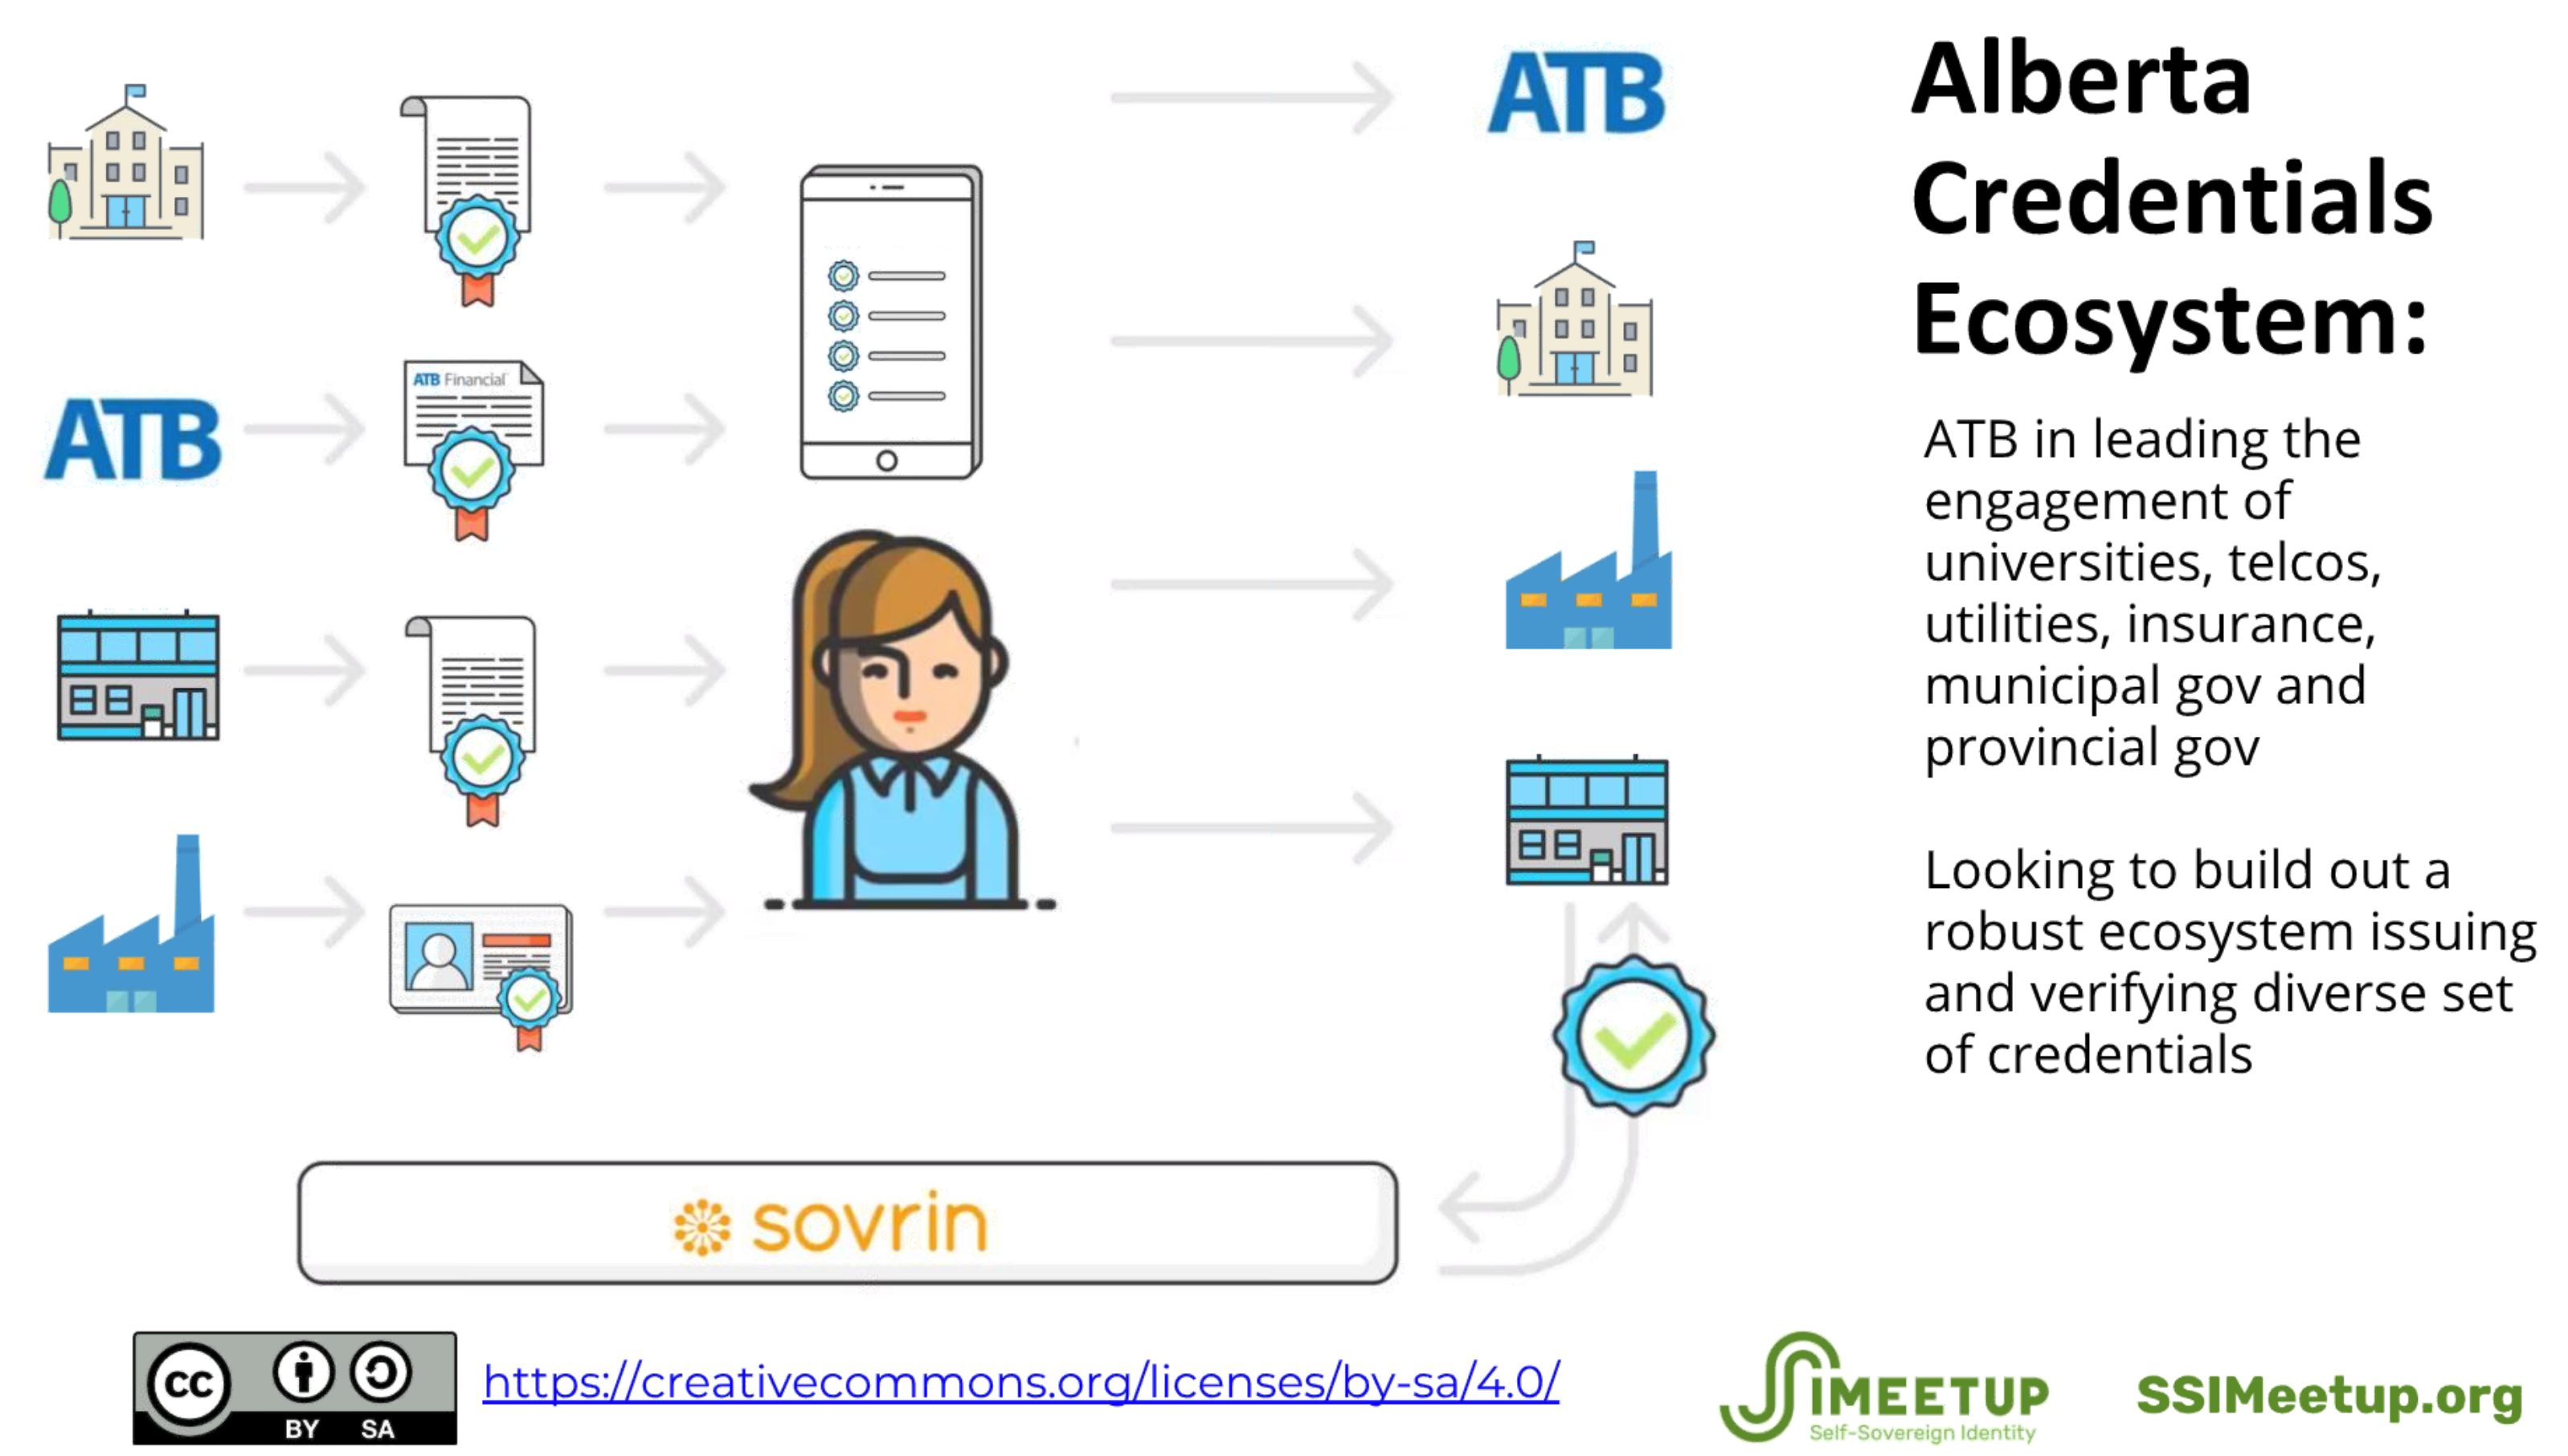
\includegraphics[height=6cm]{../pics/case_studies/alberta-credentials-ecosystem}
		\captionsetup{justification=centering}
		\caption{from \cite{ssimeetup201902:atb-slides}}
	\end{figure}
}


%----------------------------------------------------------------------------
\subsection{Use-cases in Supply Chain}
\frame{
	\frametitle{A Token can represent anything}
	\begin{figure}
		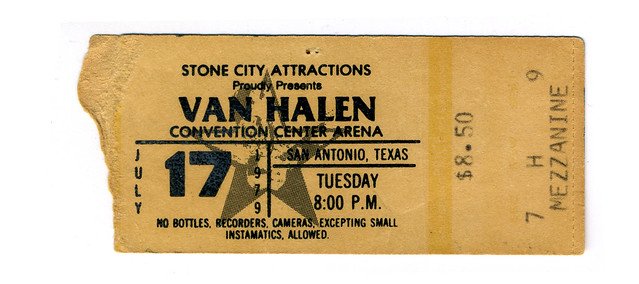
\includegraphics[width=11cm]{../pics/tokenization/ticket-van-halen}
		\captionsetup{justification=centering}
		\caption{Credit~: \href{https://www.flickr.com/photos/hmk/2121424630}{H. Michael Karshis}}
	\end{figure}
}

\frame{
	\frametitle{Native Currency}
	\begin{figure}
		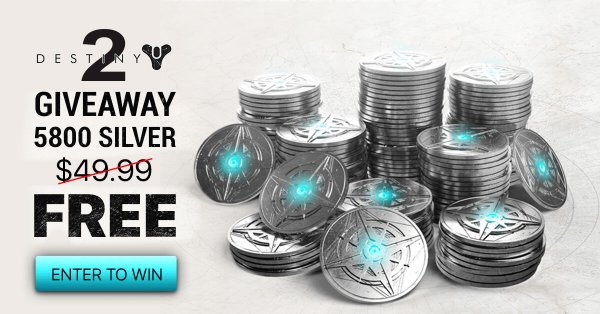
\includegraphics[height=6cm]{../pics/tokenization/destiny-silver}
		\captionsetup{justification=centering}
		\caption{Source~: give.zone (also sold on Amazon, PlayStation store, etc)}
	\end{figure}
}

\frame{
	\frametitle{Case Study: Gold tokenization}
	\begin{figure}
		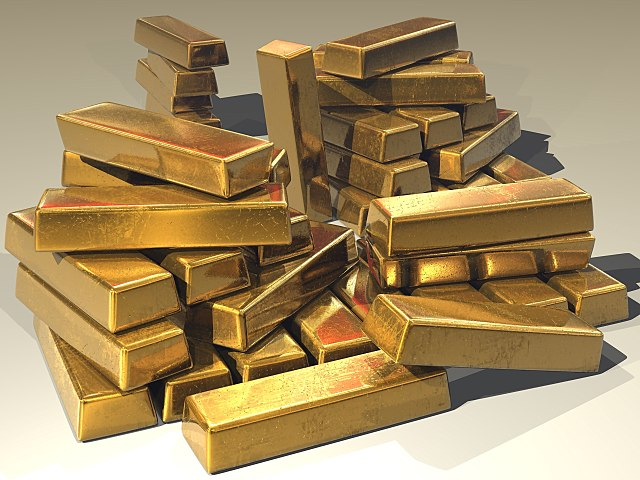
\includegraphics[height=3cm]{../pics/tokenization/640px-Gold_bullion_bars}
		\captionsetup{justification=centering}
		\caption{Credit~: \href{https://commons.wikimedia.org/wiki/File:Gold_bullion_bars.jpg}{stevebidmead}}
	\end{figure}
	\begin{itemize}
		\item JP Morgan tokenizes Gold (\cite{thetokenist2019:jpmorgangold})
		\item LAToken partners with MyGold (\cite{latoken2017:gold})
		\item \ldots 
	\end{itemize}
}

\frame{
	\frametitle{Case Studies: fractional real estate and track \& trace (Tuna)}
	\begin{figure}
		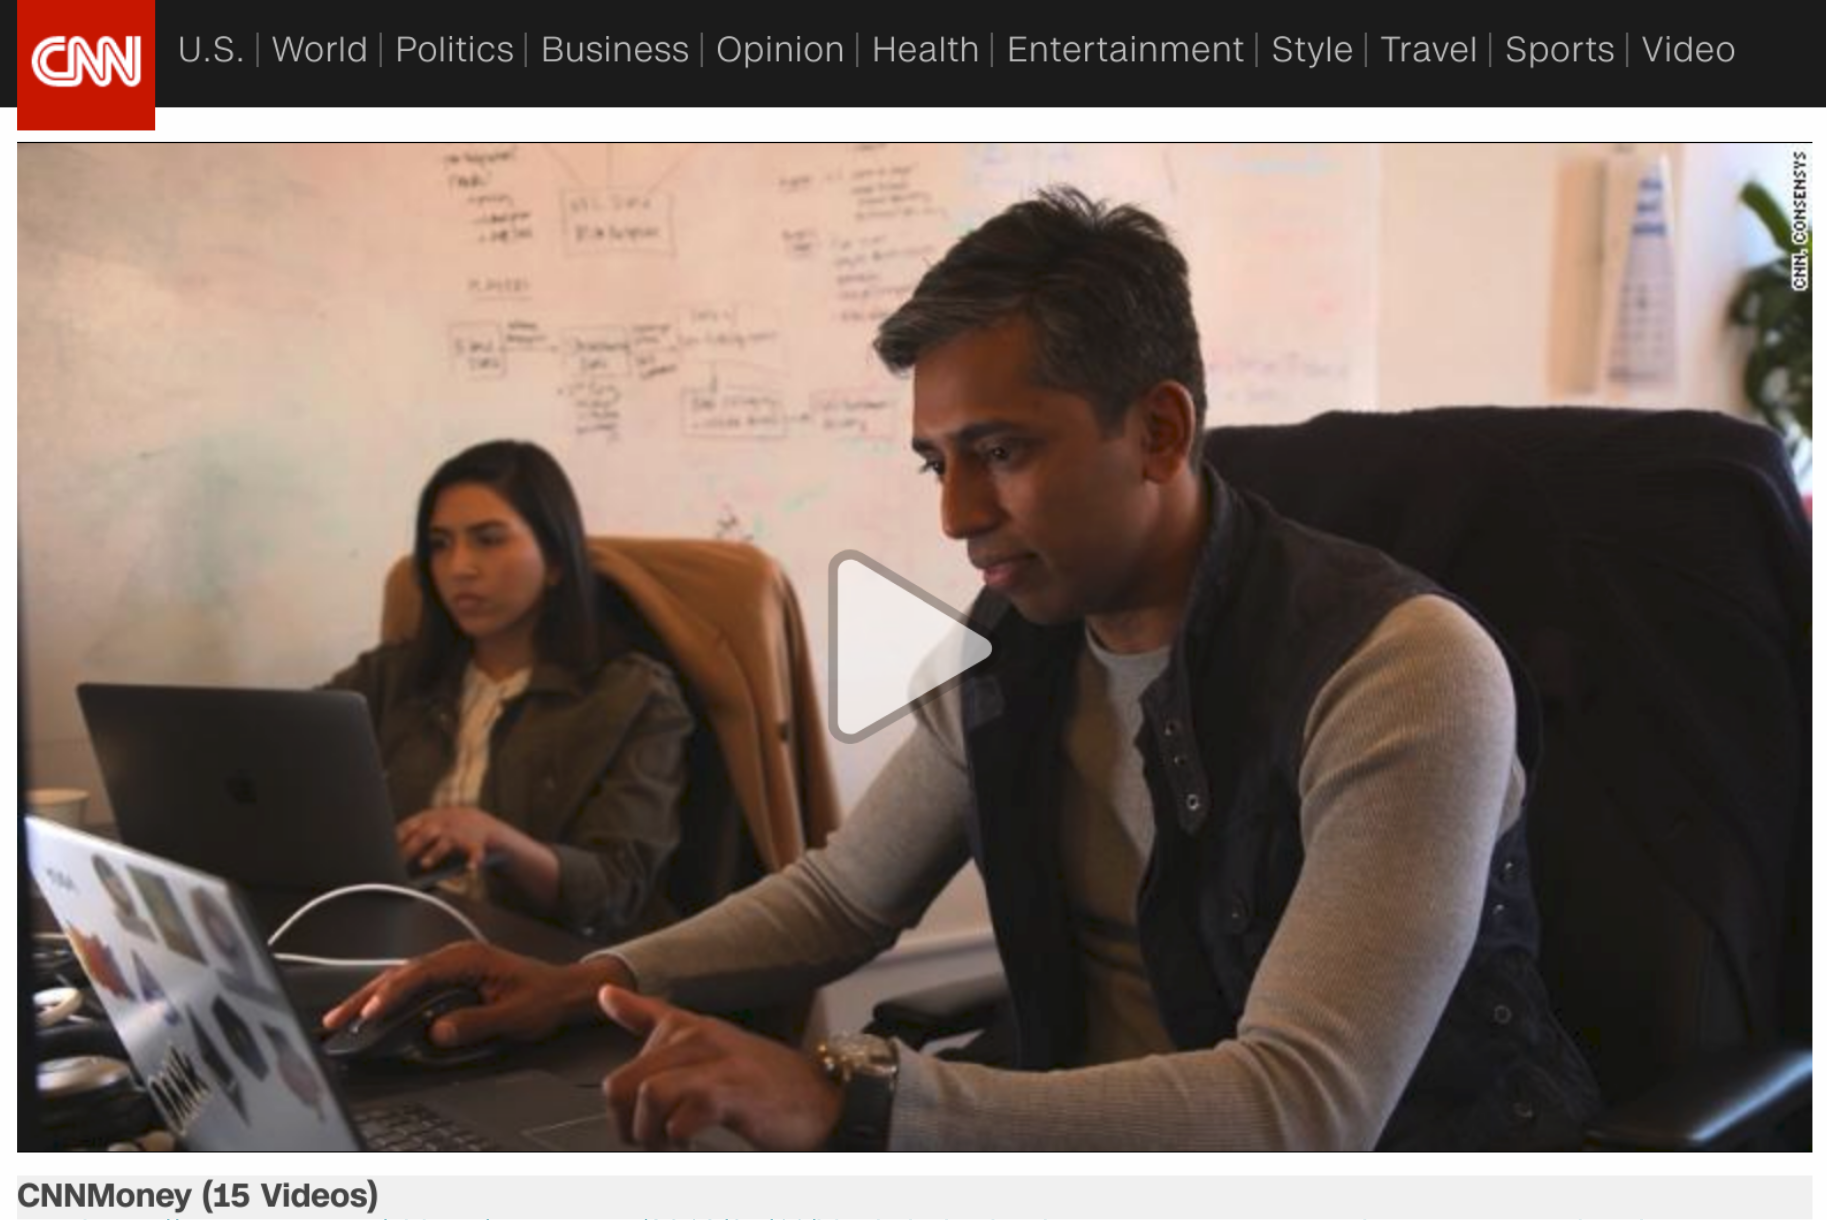
\includegraphics[height=6cm]{../pics/ConsenSys/case_studies/cnn2018-viant-meridio}
		\captionsetup{justification=centering}
		\caption{Source~: \cite{cnn2018:viant-meridio}}
	\end{figure}
}

\frame{
	\frametitle{Case Study: Ontario farmers sell corn on Blockchain rails}
	\framesubtitle{\tiny\url{https://farmtario.com/crops/ontario-farmers-make-first-blockchain-system-corn-sale/}}
	\begin{figure}
	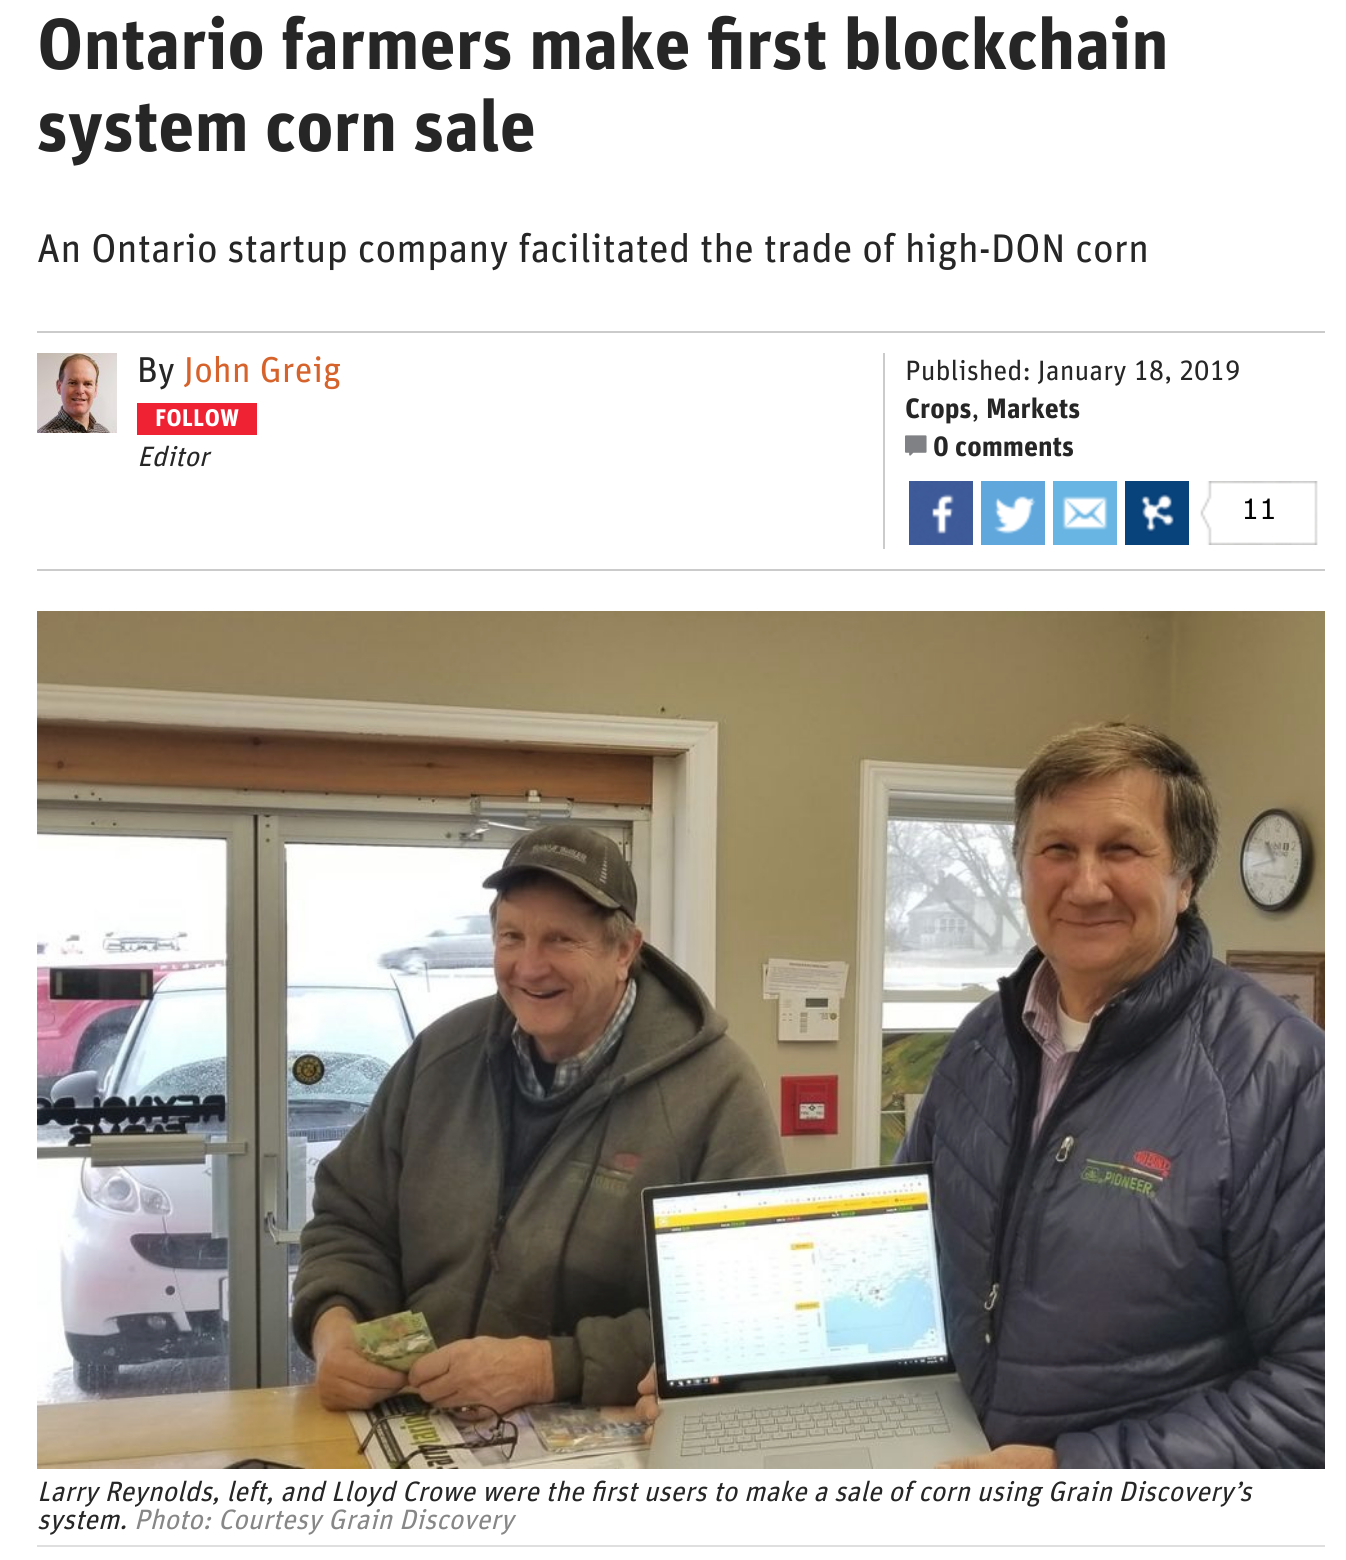
\includegraphics[height=6cm]{../pics/case_studies/ontario-farmers-corn2019}
	\end{figure}
}


%----------------------------------------------------------------------------
\subsection{Use-cases in Data and Analytics}
\frame{
	\frametitle{Alethio}
	\framesubtitle{Big Data and Analytics on Ethereum}
	\begin{figure}
		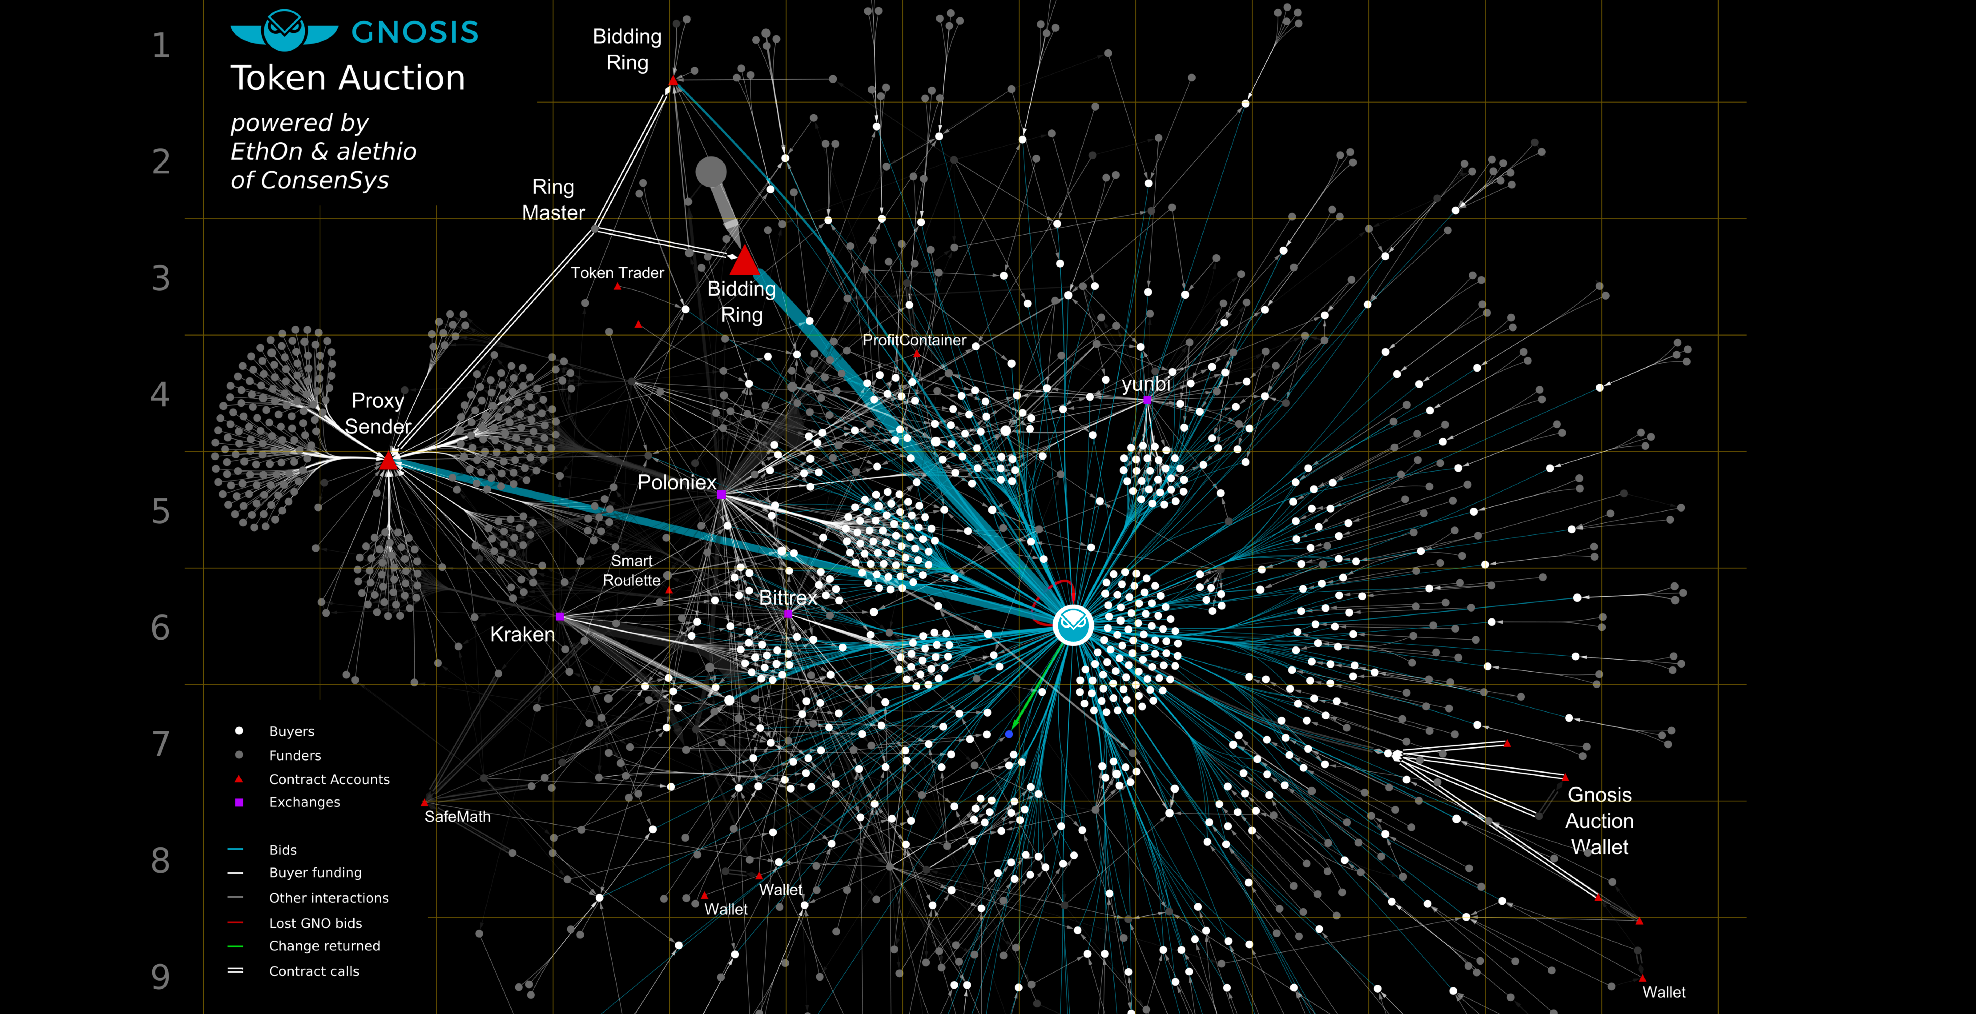
\includegraphics[width=11cm]{../pics/ConsenSys/alethio-tracking-viz}
		\caption{\url{https://aleth.io}}
	\end{figure}
}

\frame{
	\frametitle{dfuse}
	\framesubtitle{Querying the blockchain (currently available for EOS and Ethereum)}
	\begin{figure}
		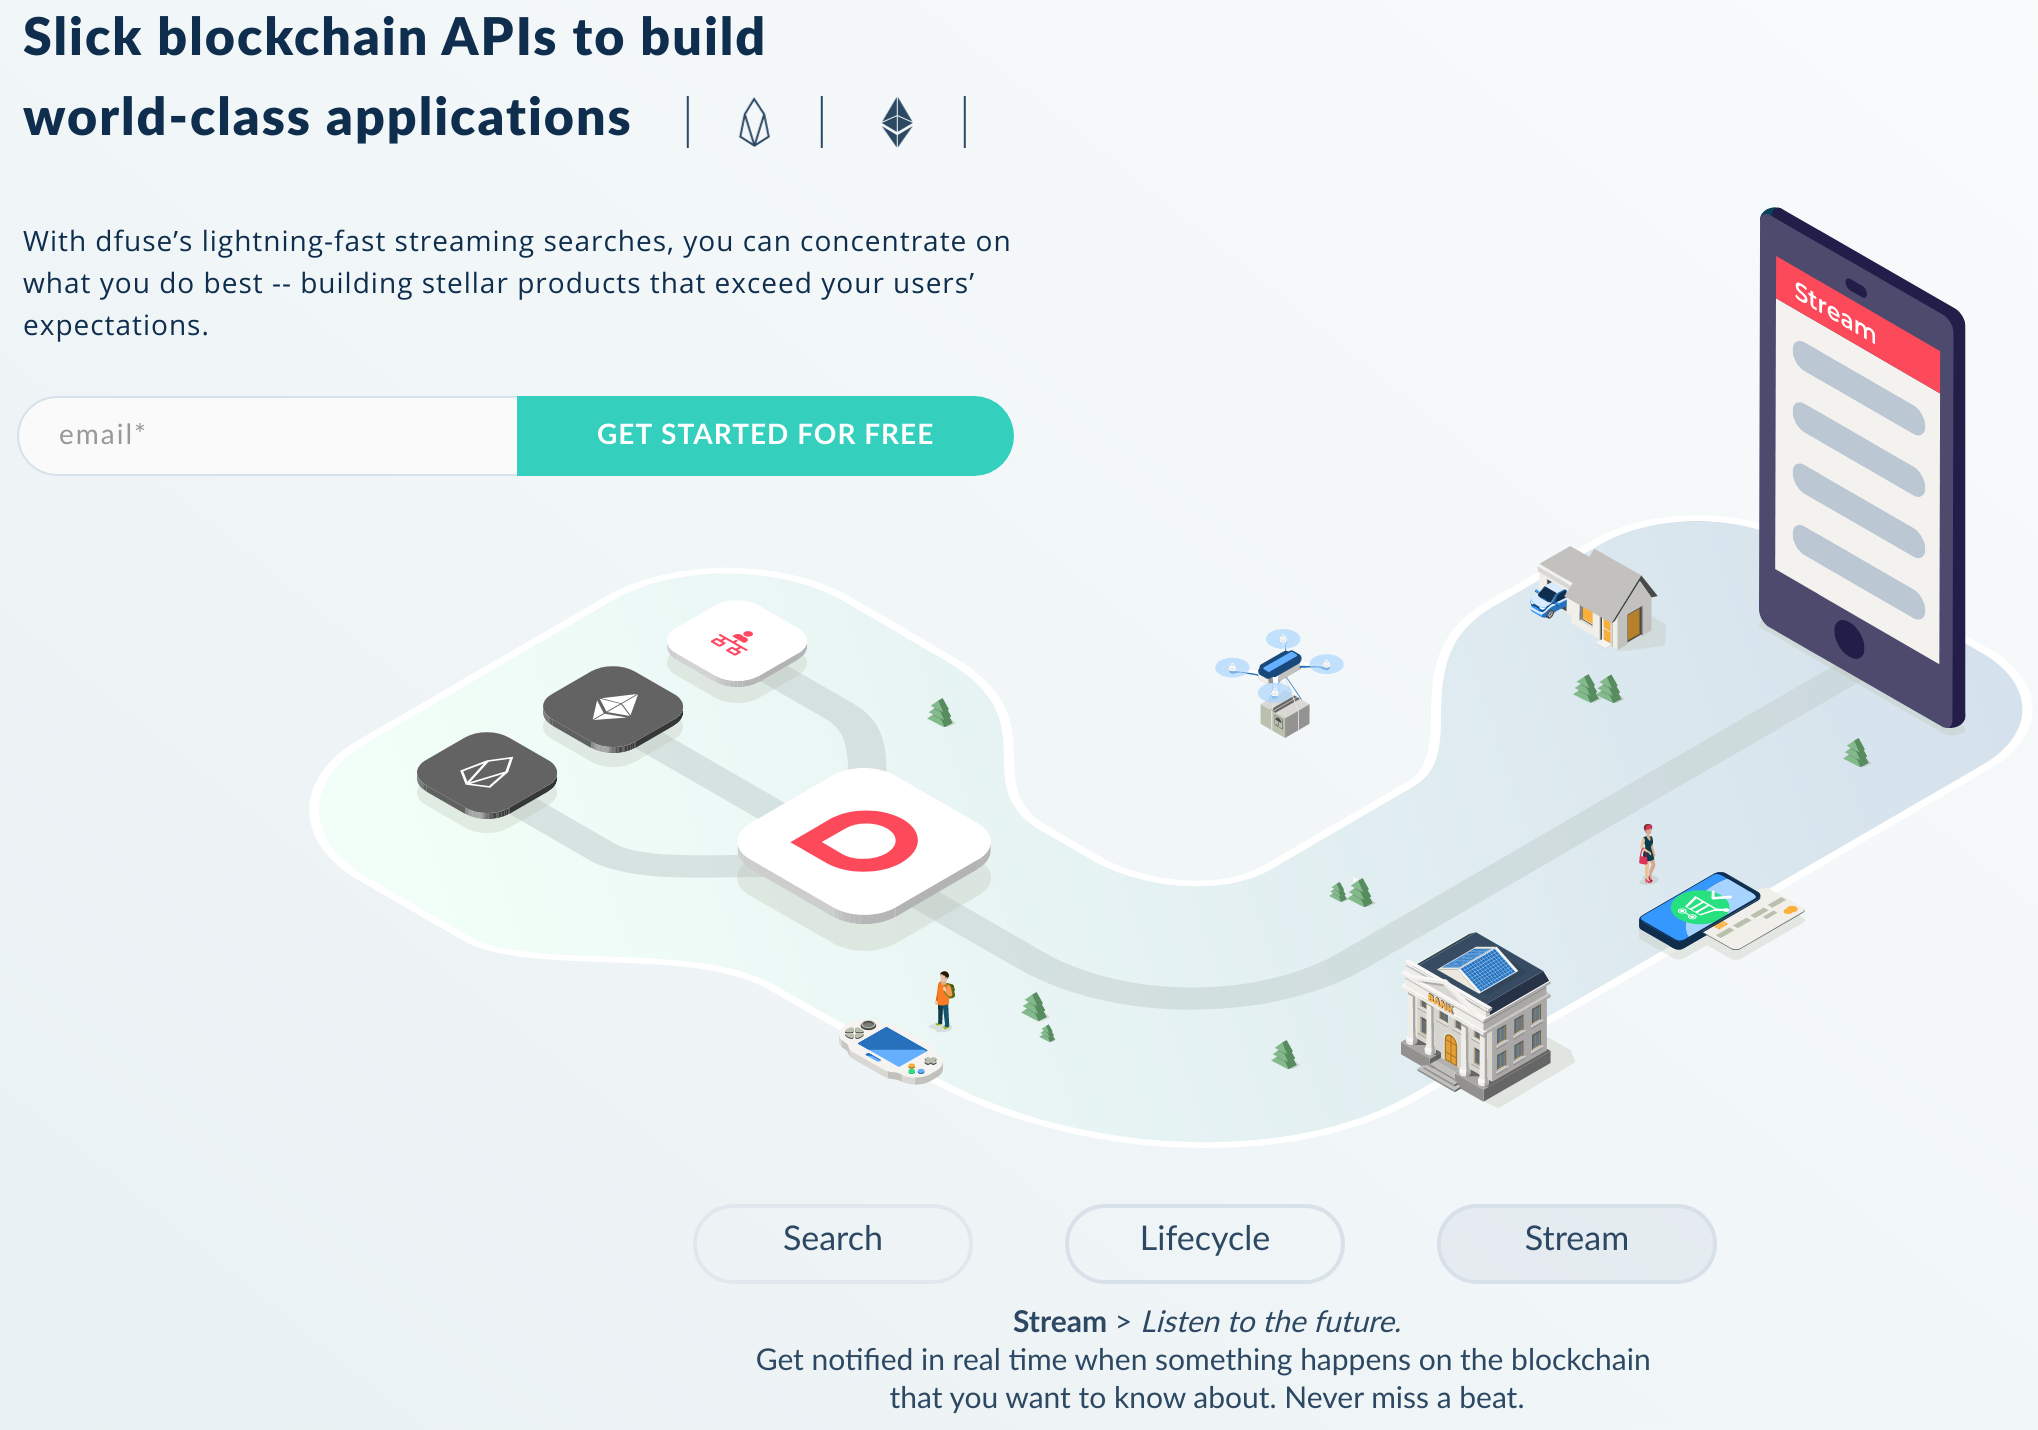
\includegraphics[width=10.5cm]{../pics/blockchain/dfuse-valueprop}
		\caption{\url{https://dfuse.io}}
	\end{figure}
}

%----------------------------------------------------------------------------
\subsection{Use-cases in Media \& Entertainment}
\frame{
	\frametitle{Use Cases in Media \& Entertainment}
	\begin{figure}
		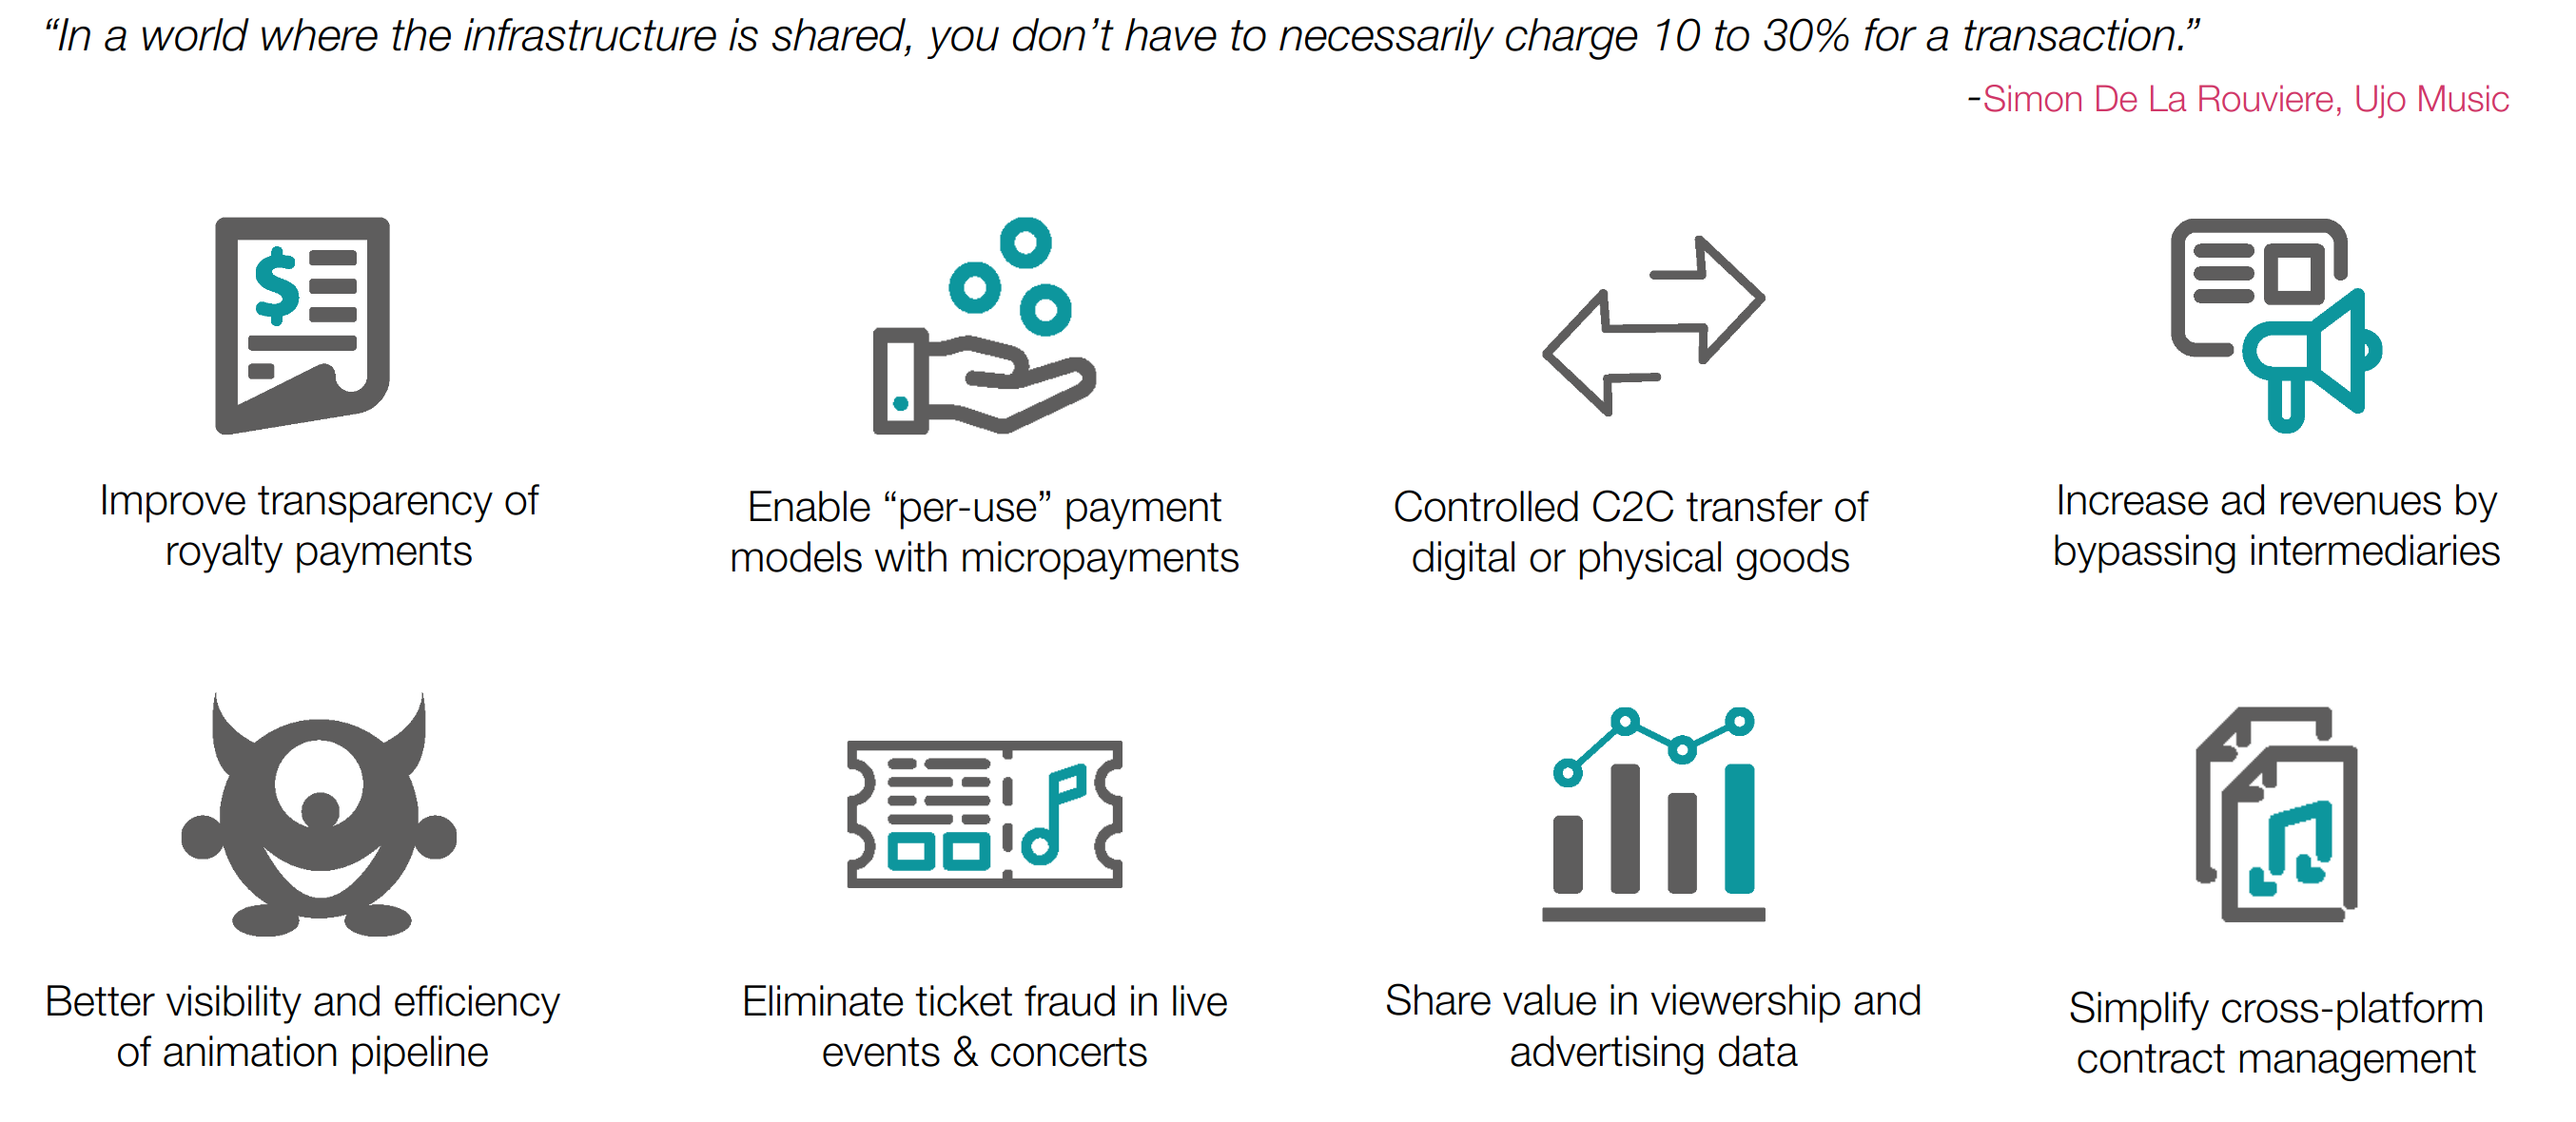
\includegraphics[width=11cm]{../pics/ConsenSys/industry/use-case-ME}
	\end{figure}
}

\frame{
	\frametitle{In Toronto: Prescient is developing an Attribution Ledger for Work of Arts}	
	\begin{figure}
		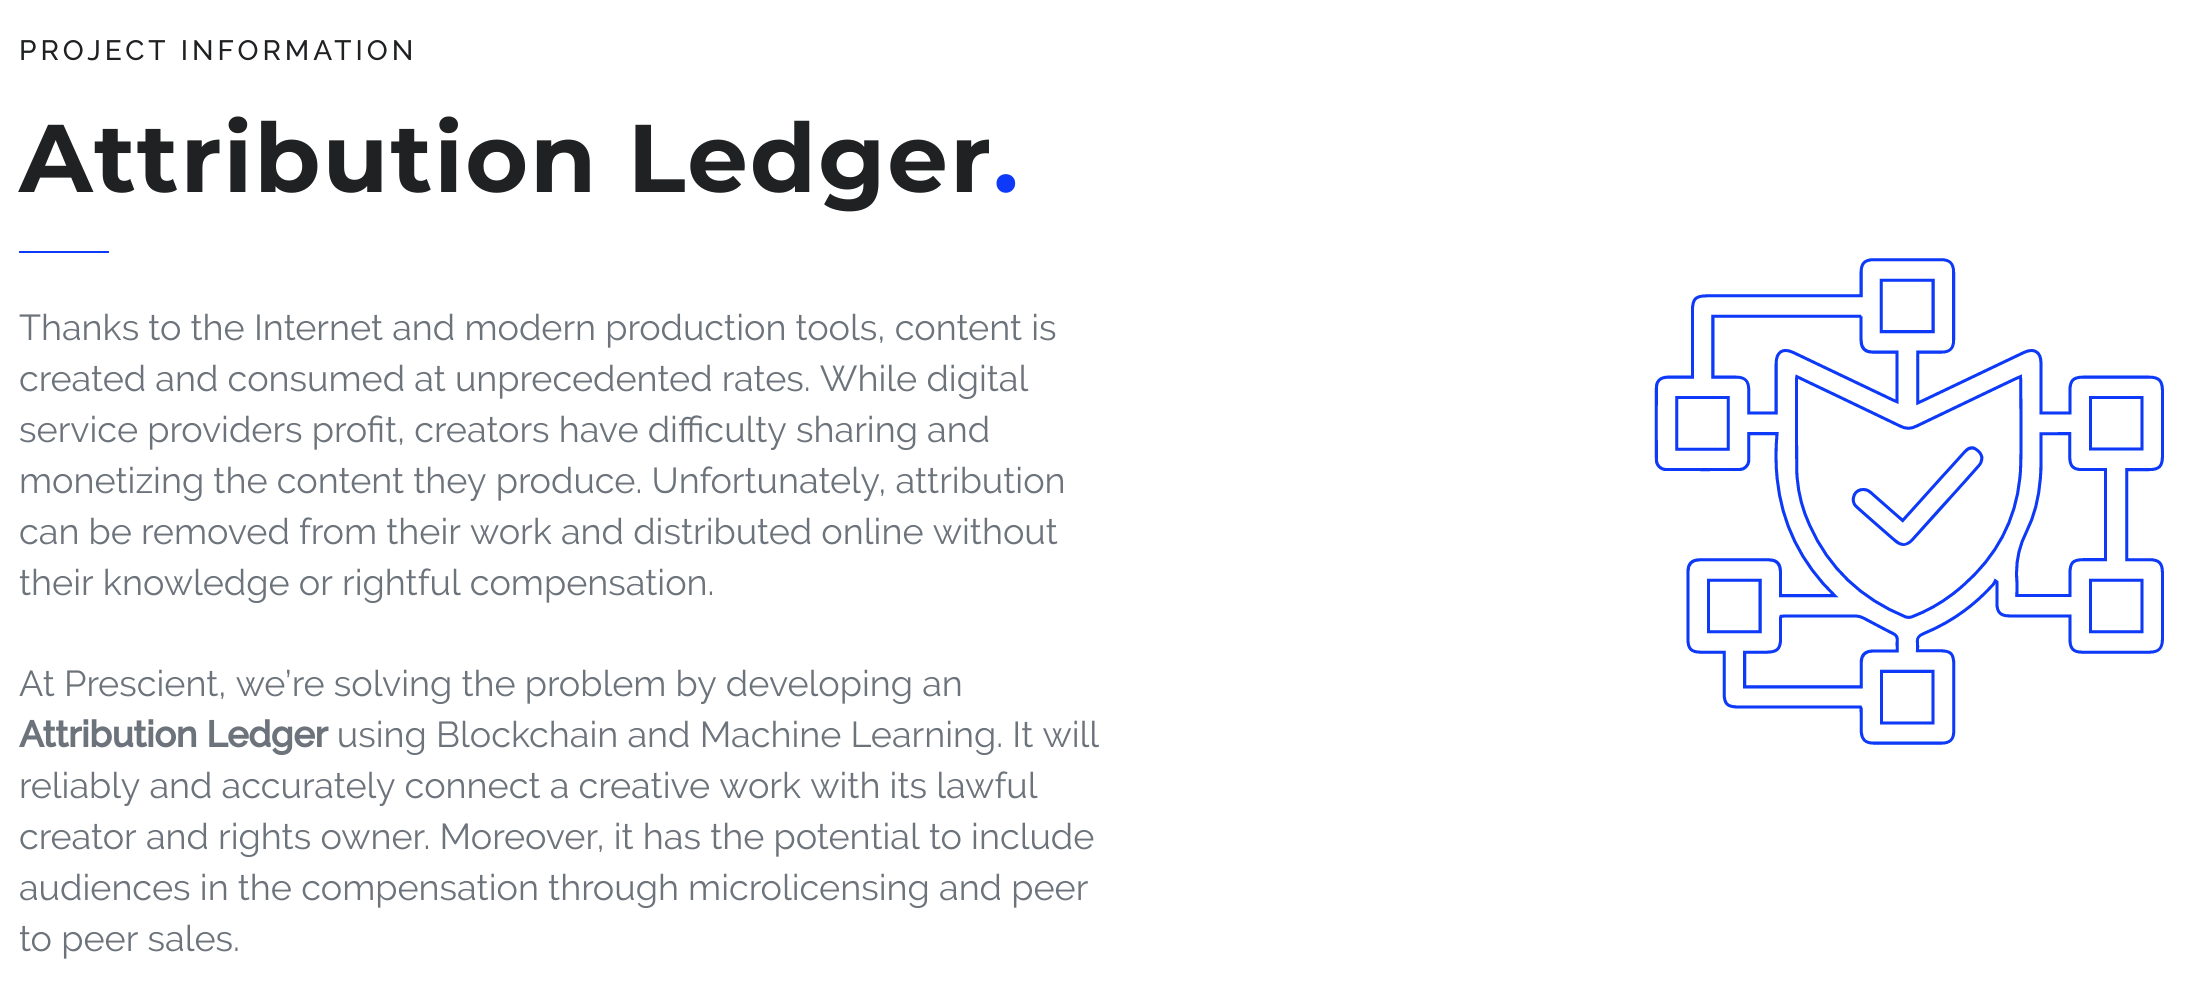
\includegraphics[width=11cm]{../pics/tokenization/prescient-attribution-ledger}
		\captionsetup{justification=centering}
		\caption{Source~: \url{https://prescientinnovations.com/attribution-ledger}}
	\end{figure}
}

\begin{frame}   
	\frametitle{Case study: Berntein}
	\begin{figure}
		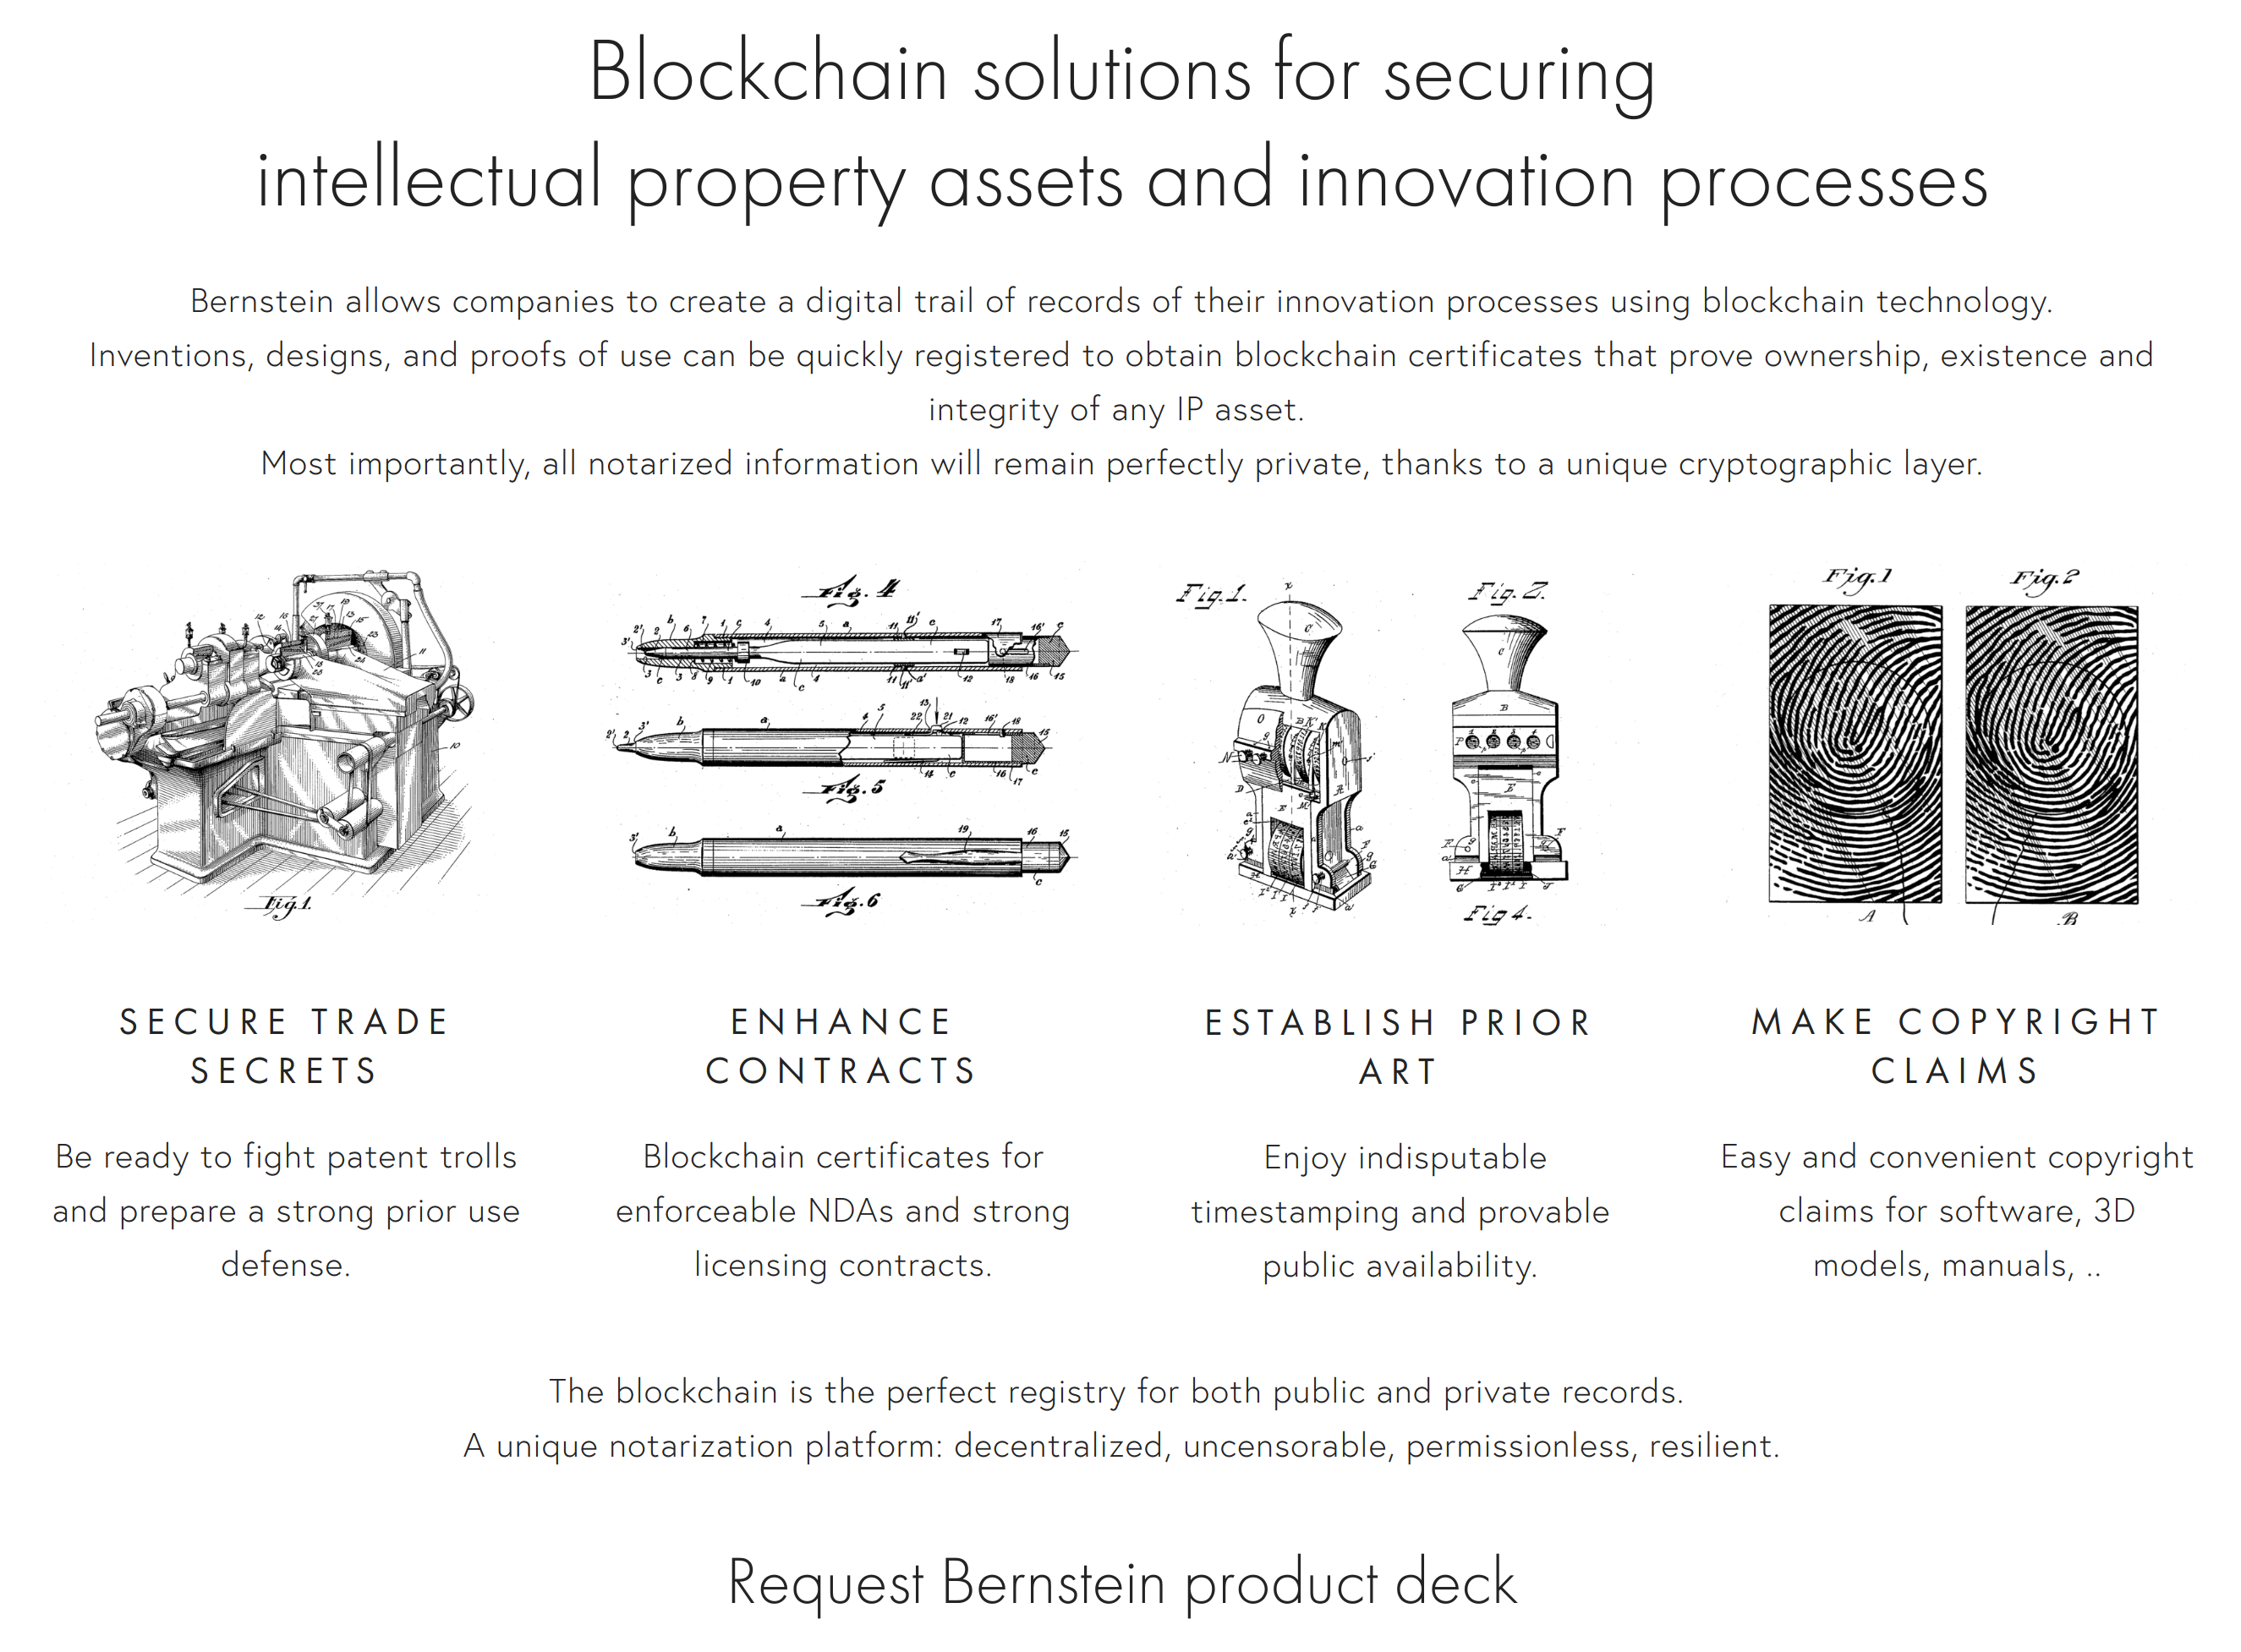
\includegraphics[width=10cm]{../pics/case_studies/bernstein}
		\caption{\url{https://www.bernstein.io}}
	\end{figure}
\end{frame}

\begin{frame}   
	\frametitle{Case study: Vaultitude}
	\begin{figure}
		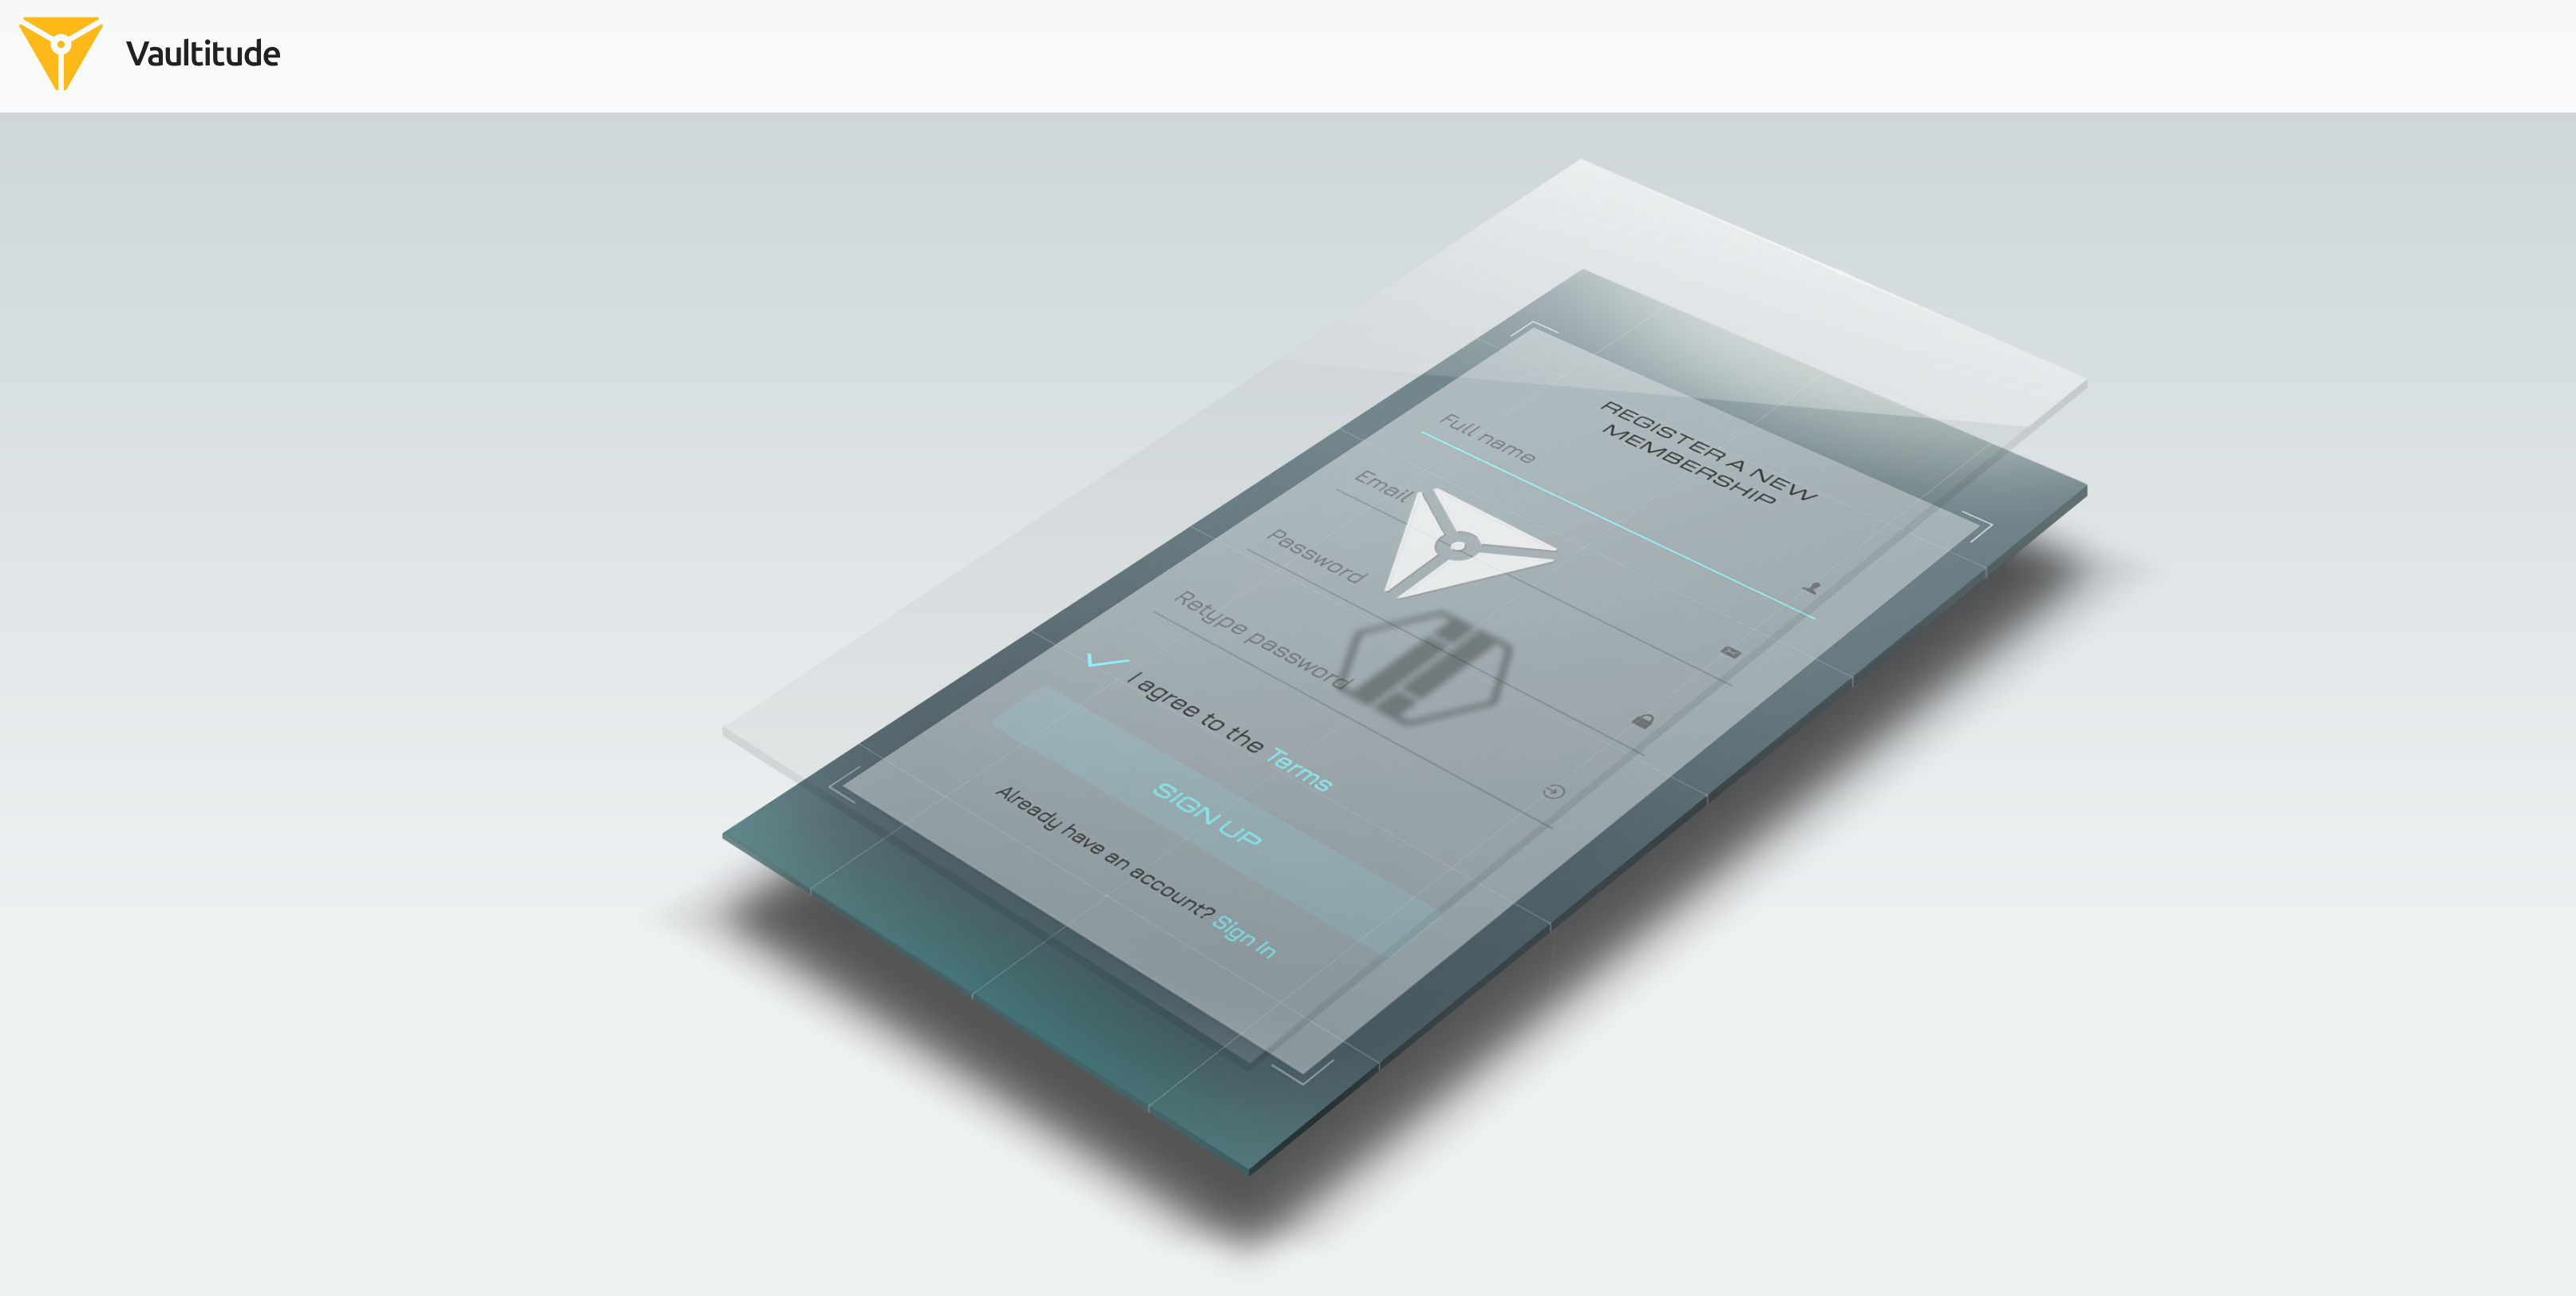
\includegraphics[width=11cm]{../pics/case_studies/vaultitude}
		\caption{\url{https://vaultitude.com}}
	\end{figure}
\end{frame}

\begin{frame}   
	\frametitle{Case study: Baoquan}
	\begin{figure}
		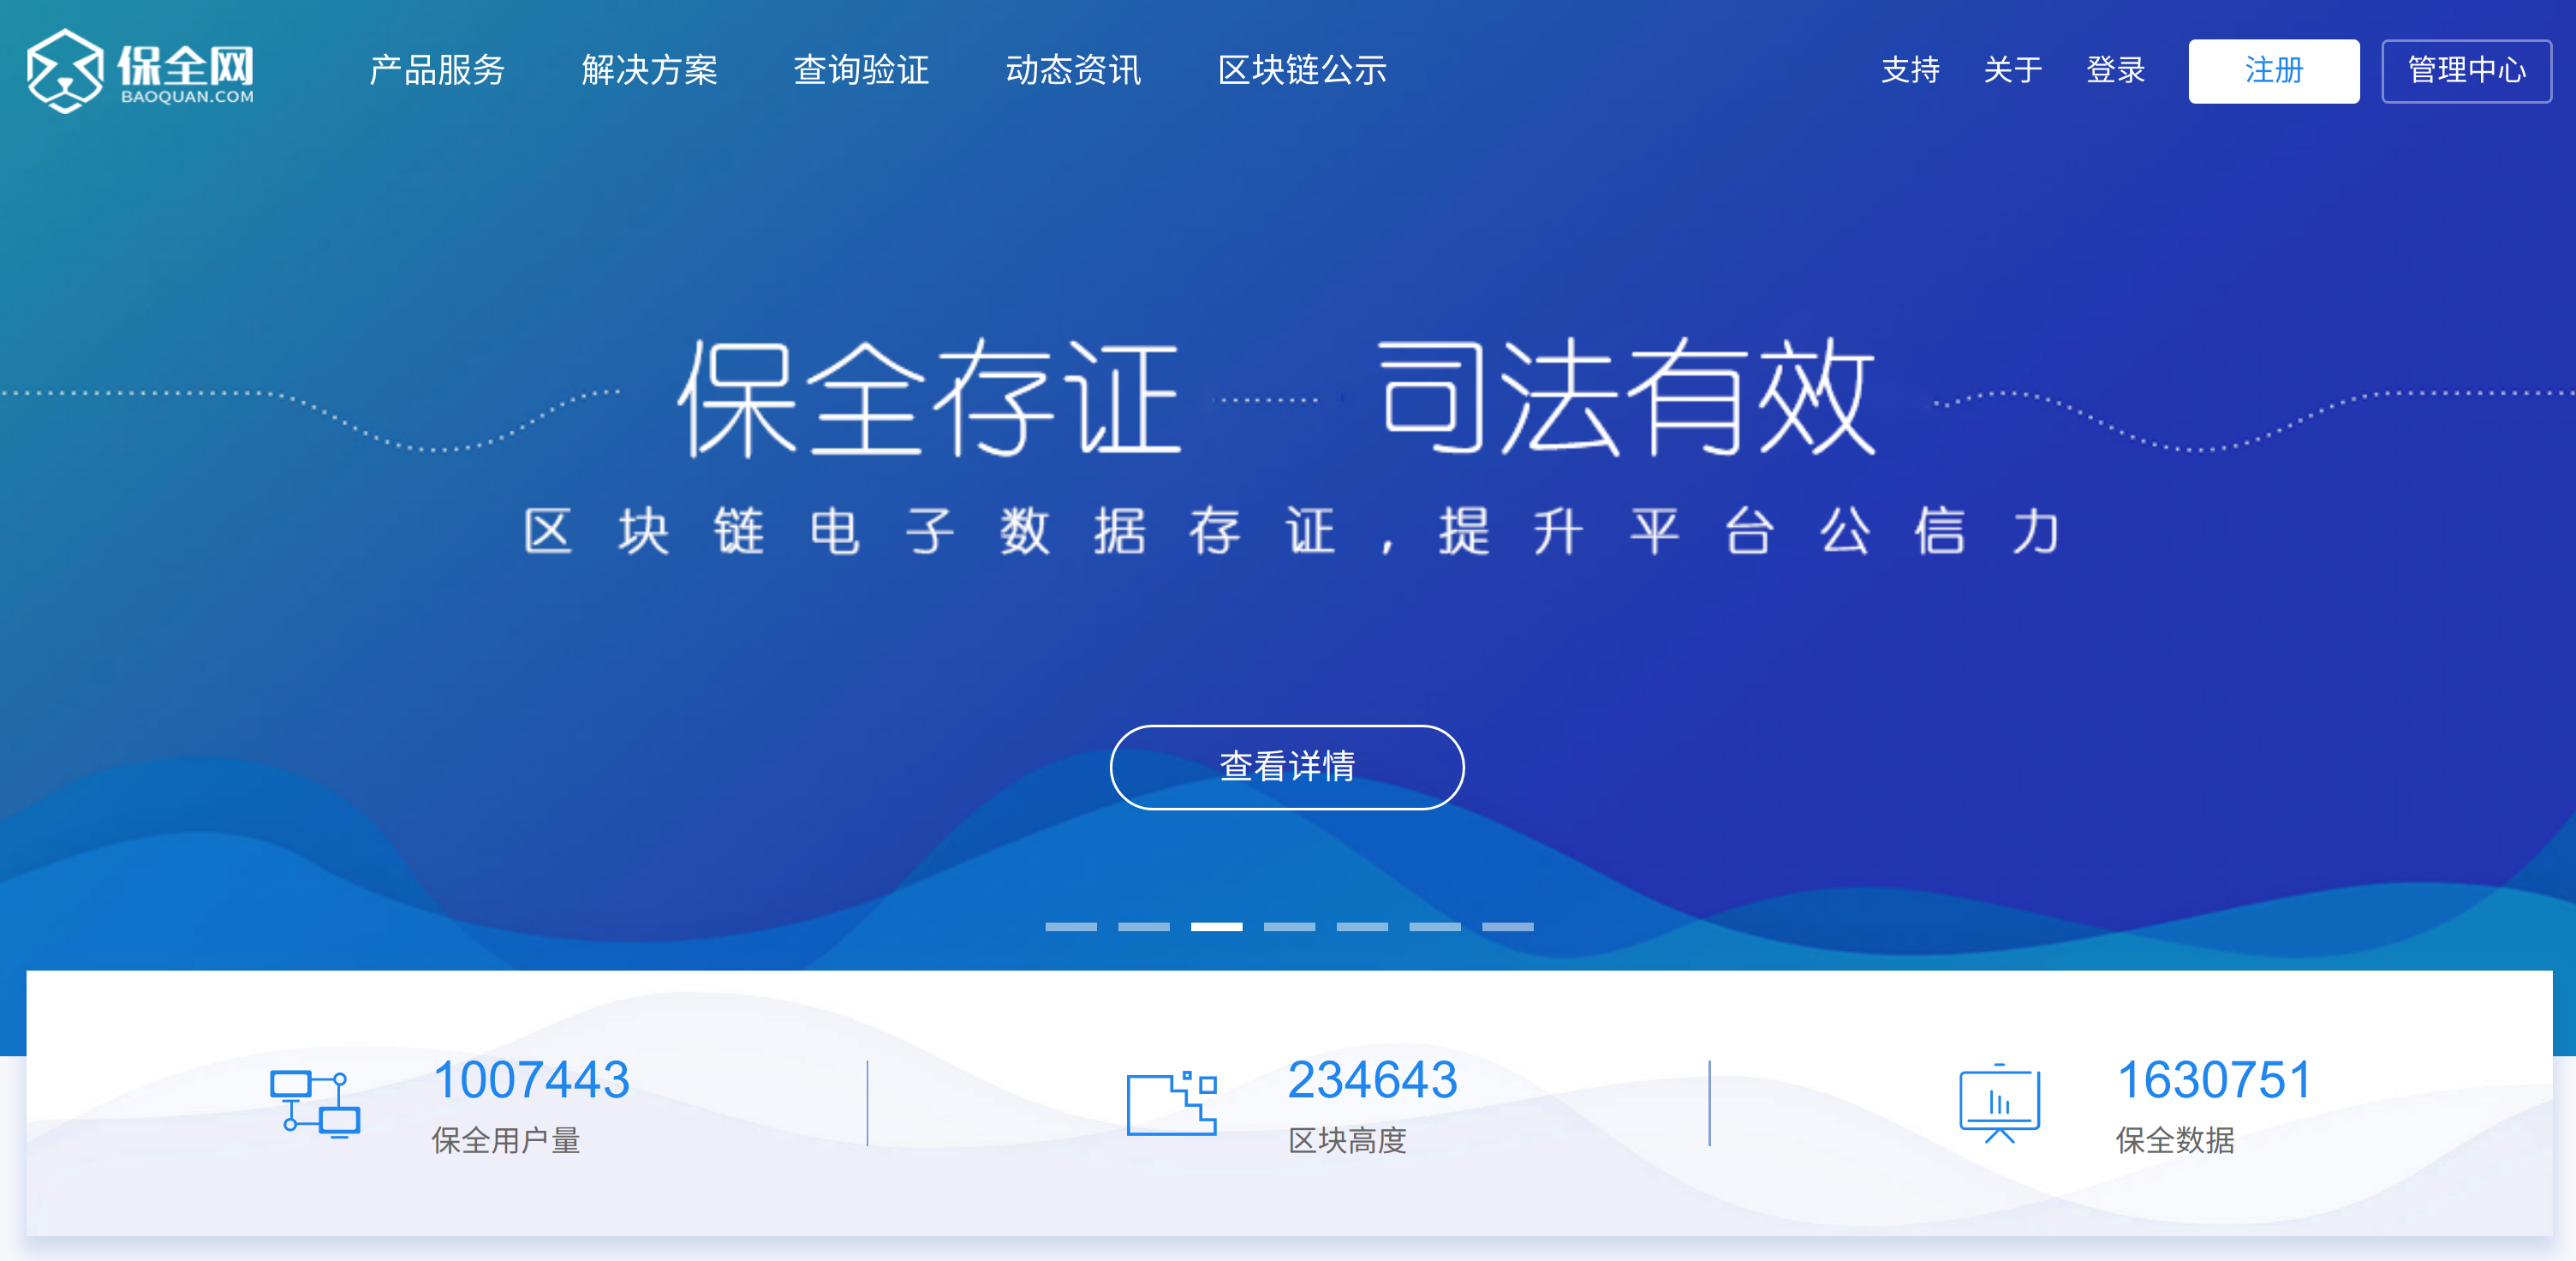
\includegraphics[width=11cm]{../pics/case_studies/baoquan}
		\caption{The Hangzhou Internet Court accepted evidence from the Baoquan Blockchain on a copyright case (\cite{chinesecourt2018})}
	\end{figure}
\end{frame}


\frame{
	\frametitle{Token-Curated Registry Pattern}
	\begin{figure}
		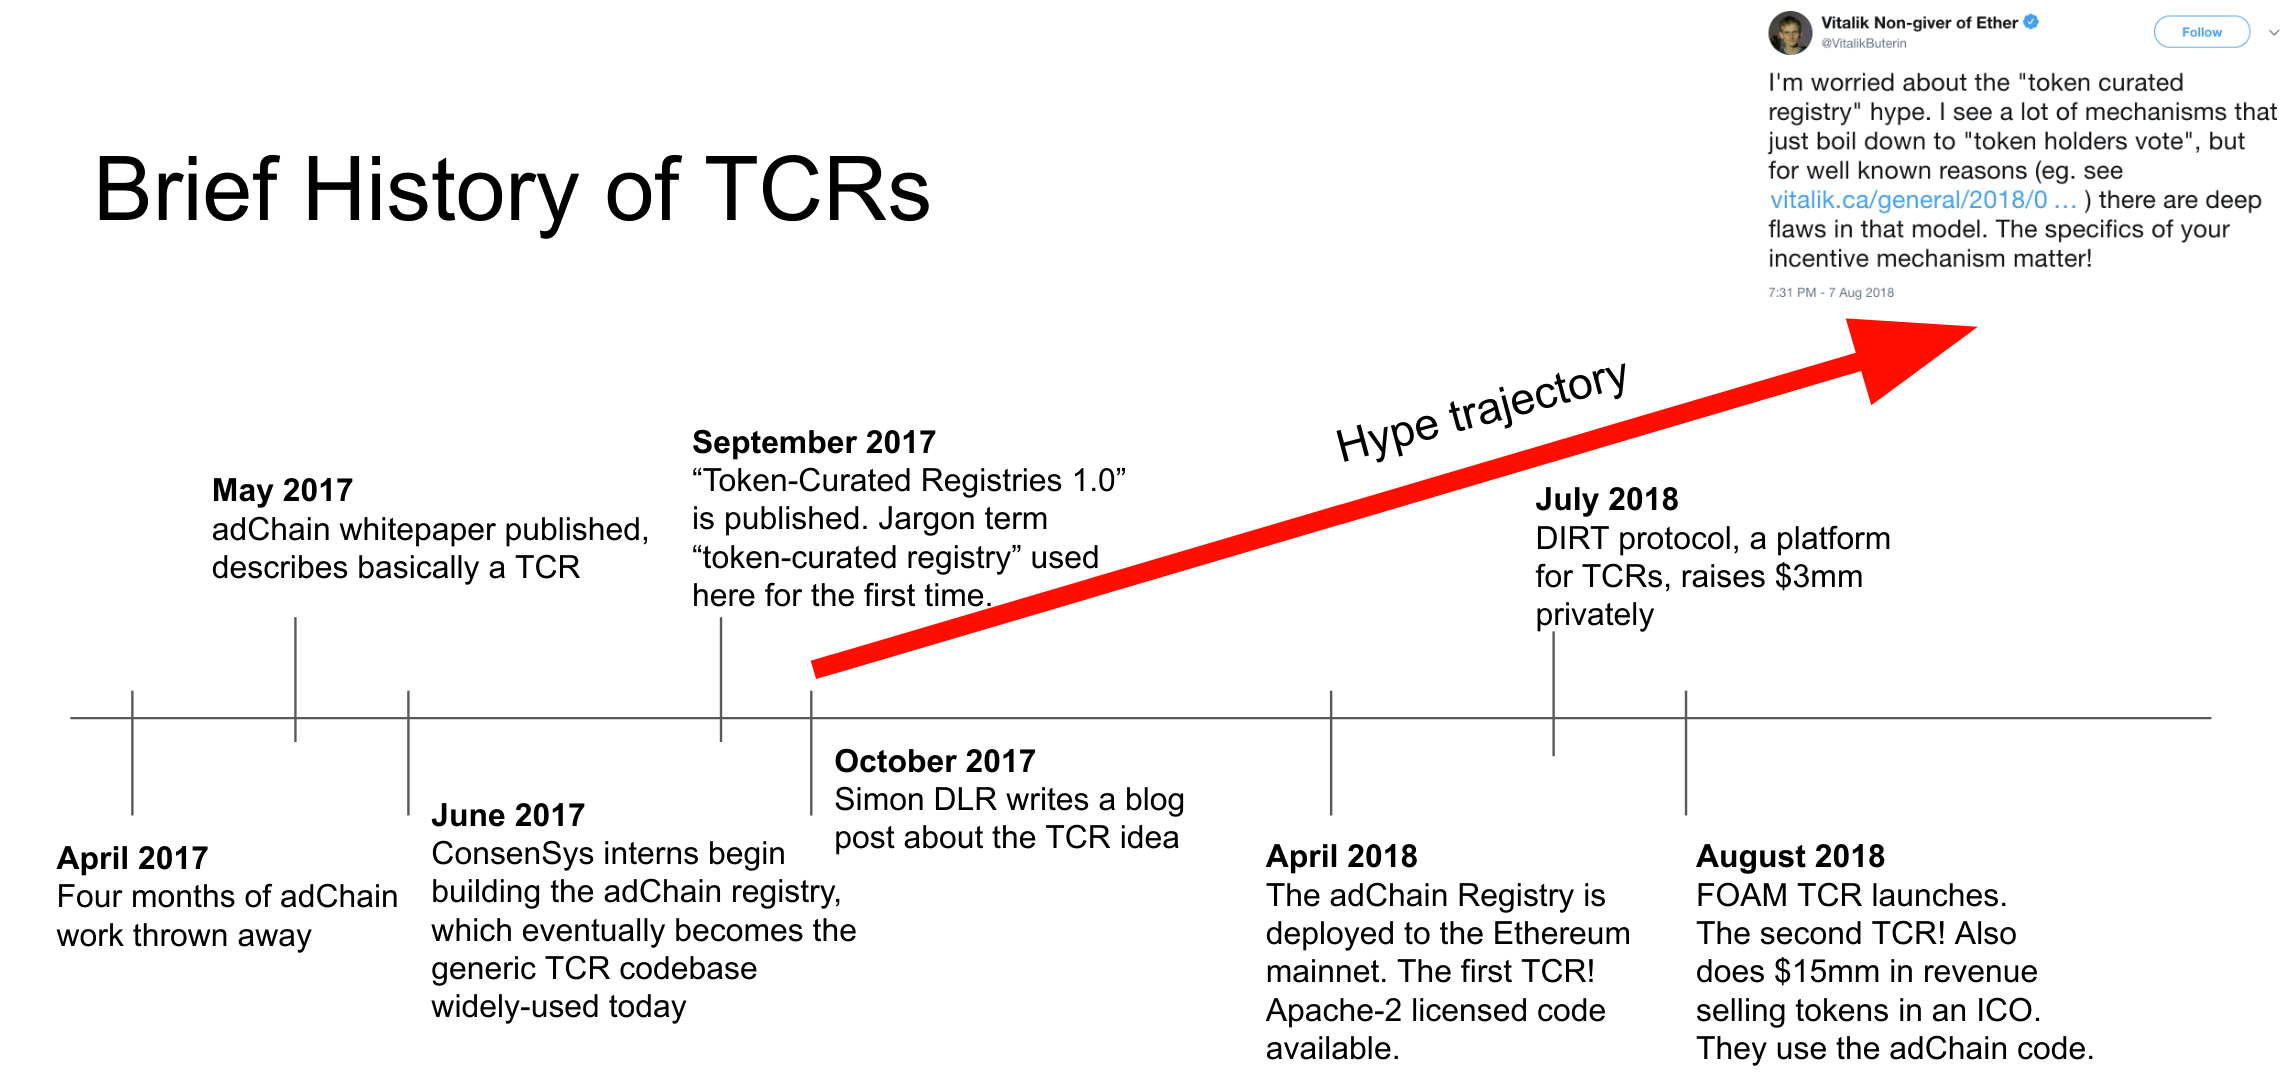
\includegraphics[width=11cm]{../pics/ConsenSys/Design_Patterns/TCR_history_2018H1}
		\caption{from Mike \citeauthor{mikegoldin2018:tcrprezi}'s presentation (\citeyear{mikegoldin2018:tcrprezi})}
	\end{figure}
}


\frame{
	\frametitle{Developer-friendly marketplace: The Bounties Network}
	\framesubtitle{Why not getting paid for your work?}
	\begin{figure}
		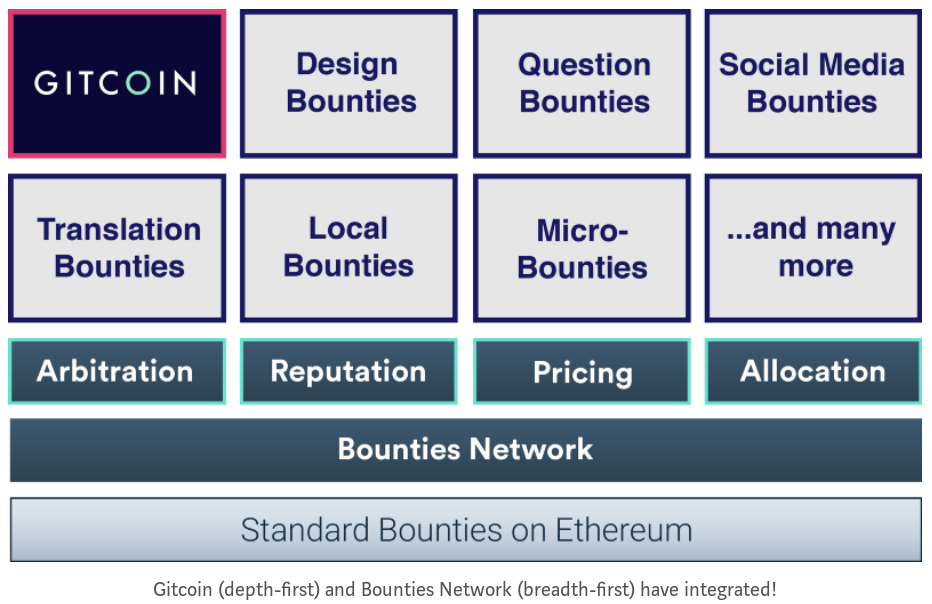
\includegraphics[width=11cm]{../pics/ConsenSys/bounties_network_stack}
		\framesubtitle{\url{https://bounties.network}}
	\end{figure}
}

\frame{
	\frametitle{Gitcoin}
	\framesubtitle{Gitcoin is not a coin}
	\begin{figure}
		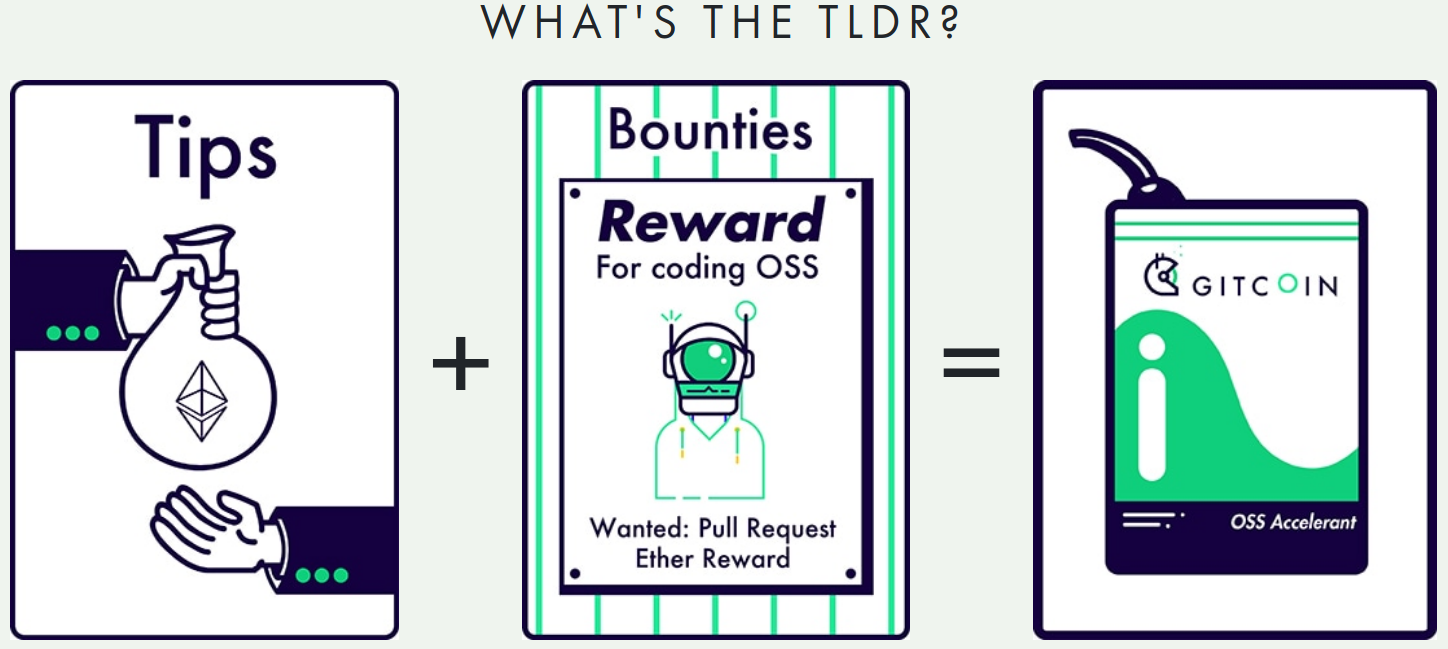
\includegraphics[width=11cm]{../pics/ConsenSys/gitcoin-tldr}
		\caption{\url{https://gitcoin.co}}
	\end{figure}
}








